\chapter{Results and Analysis}
% screenshots of the results - positive and negative
\section{Latent Semantic Analysis}
We experiment with multiple values of matrix rank reduction and we find that as we reduce the rank of documents-tokens matrices, they become more dense. As we reduce the ranks, the distribution of  the learnt weights also change. 

\subsection{Full-rank matrices}

Figure 13 shows the the similarity matrices computed using full-rank documents-tokens matrices for name and description and help text. We do not apply rank reduction on documents-tokens matrix of input and output file types. Using these similarity matrices, we find an optimal combination by optimizing them. The "optimal" correlation plot shows this weighted average. Figure 14 shows the distribution of weights for multiple tool attributes. We see the magnitude of weights learnt for input and output file types is higher than the other two. It is associated with the higher values captured for the similarity matrix of input and output file types.

\begin{figure}[h]
\begin{centering}
    {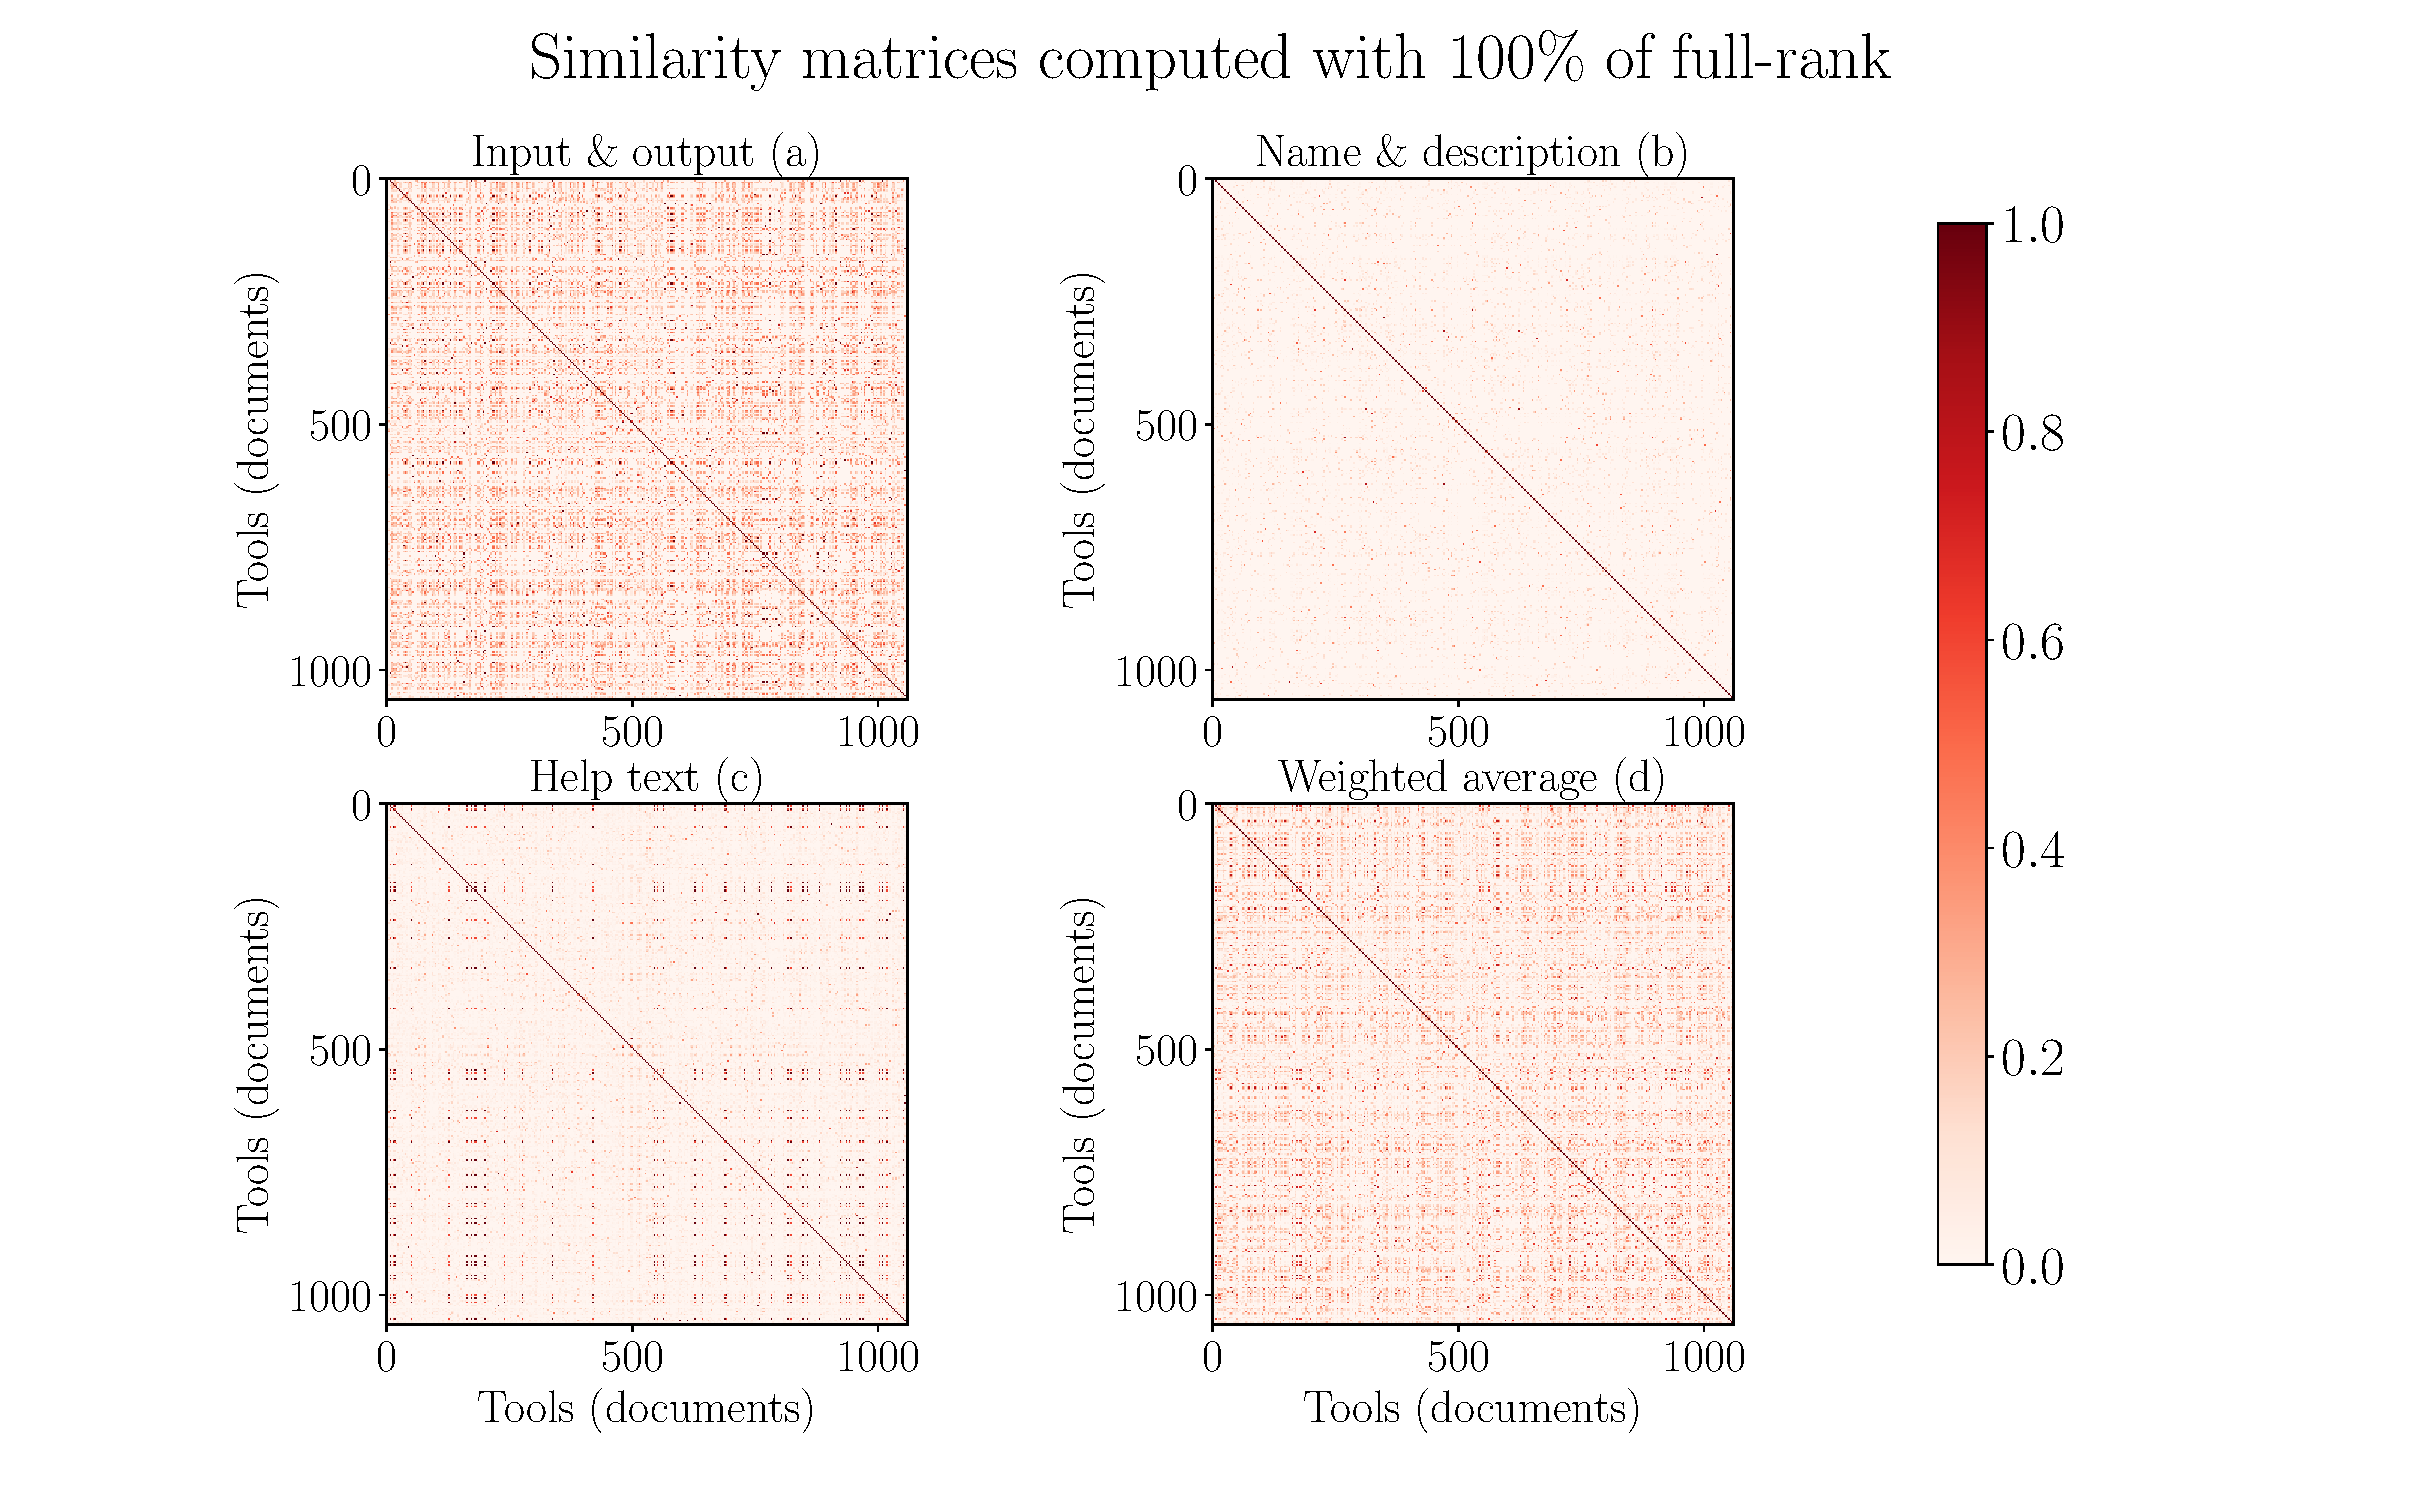
\includegraphics[scale=0.35]{figures/Similarity_matrices_100.pdf}}
    \caption[Similarity matrices full rank]{\textbf{Similarity matrices using full rank}: this correlation plot shows the individual similarity matrices for multiple attributes and the weighted average of these matrices as optimal one.}
\end{centering}
\end{figure}

\begin{figure}[h]
\begin{centering}
    {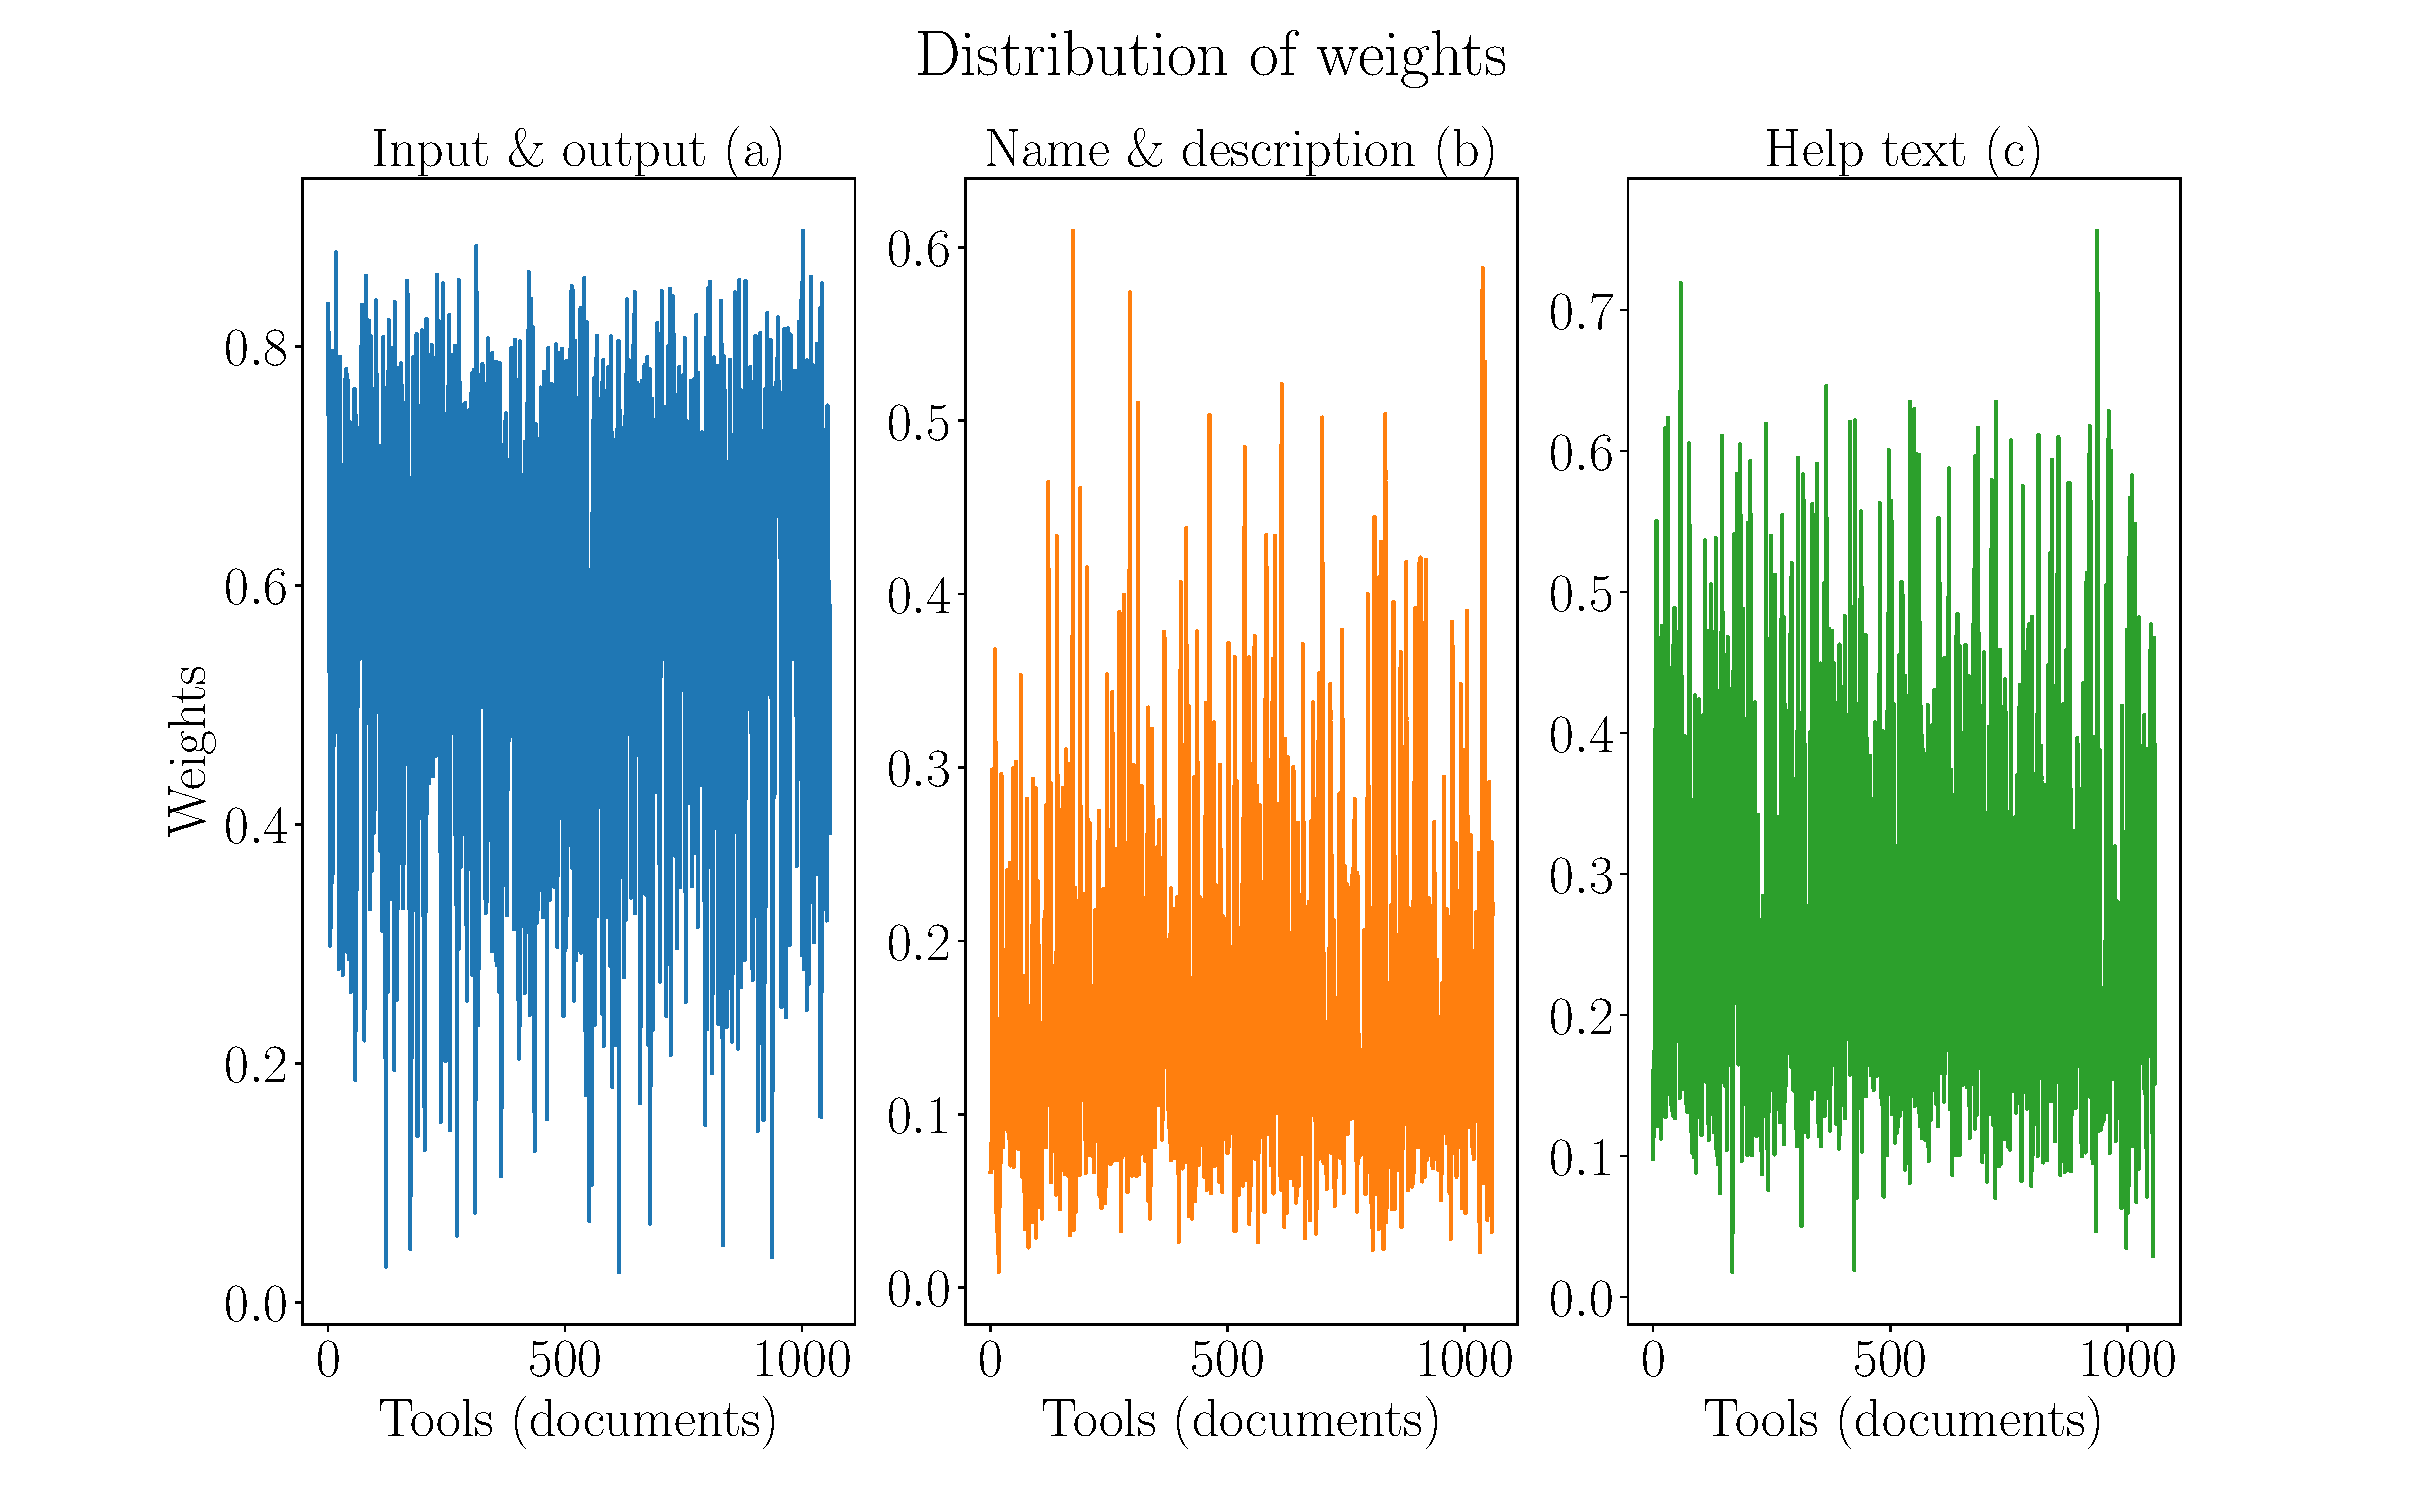
\includegraphics[scale=0.35]{figures/Weights_100.pdf}}
    \caption[Weights distribution full rank]{\textbf{Weights distribution full rank}: this plot show how the weights vary for multiple tool attributes.}
\end{centering}
\end{figure}

\subsection{70\% of full-rank}
We reduce the ranks of two documents-tokens matrices to 70\% of the original ranks. For example, if the rank of a matrix is 100, we reduce the rank to 70 using singular value decomposition. From figure 15, we see that the name and description and help text similarity matrices start becoming more dense compared to figure 13. The distribution of the weights also change (figure 16).

\begin{figure}[h]
\begin{centering}
    {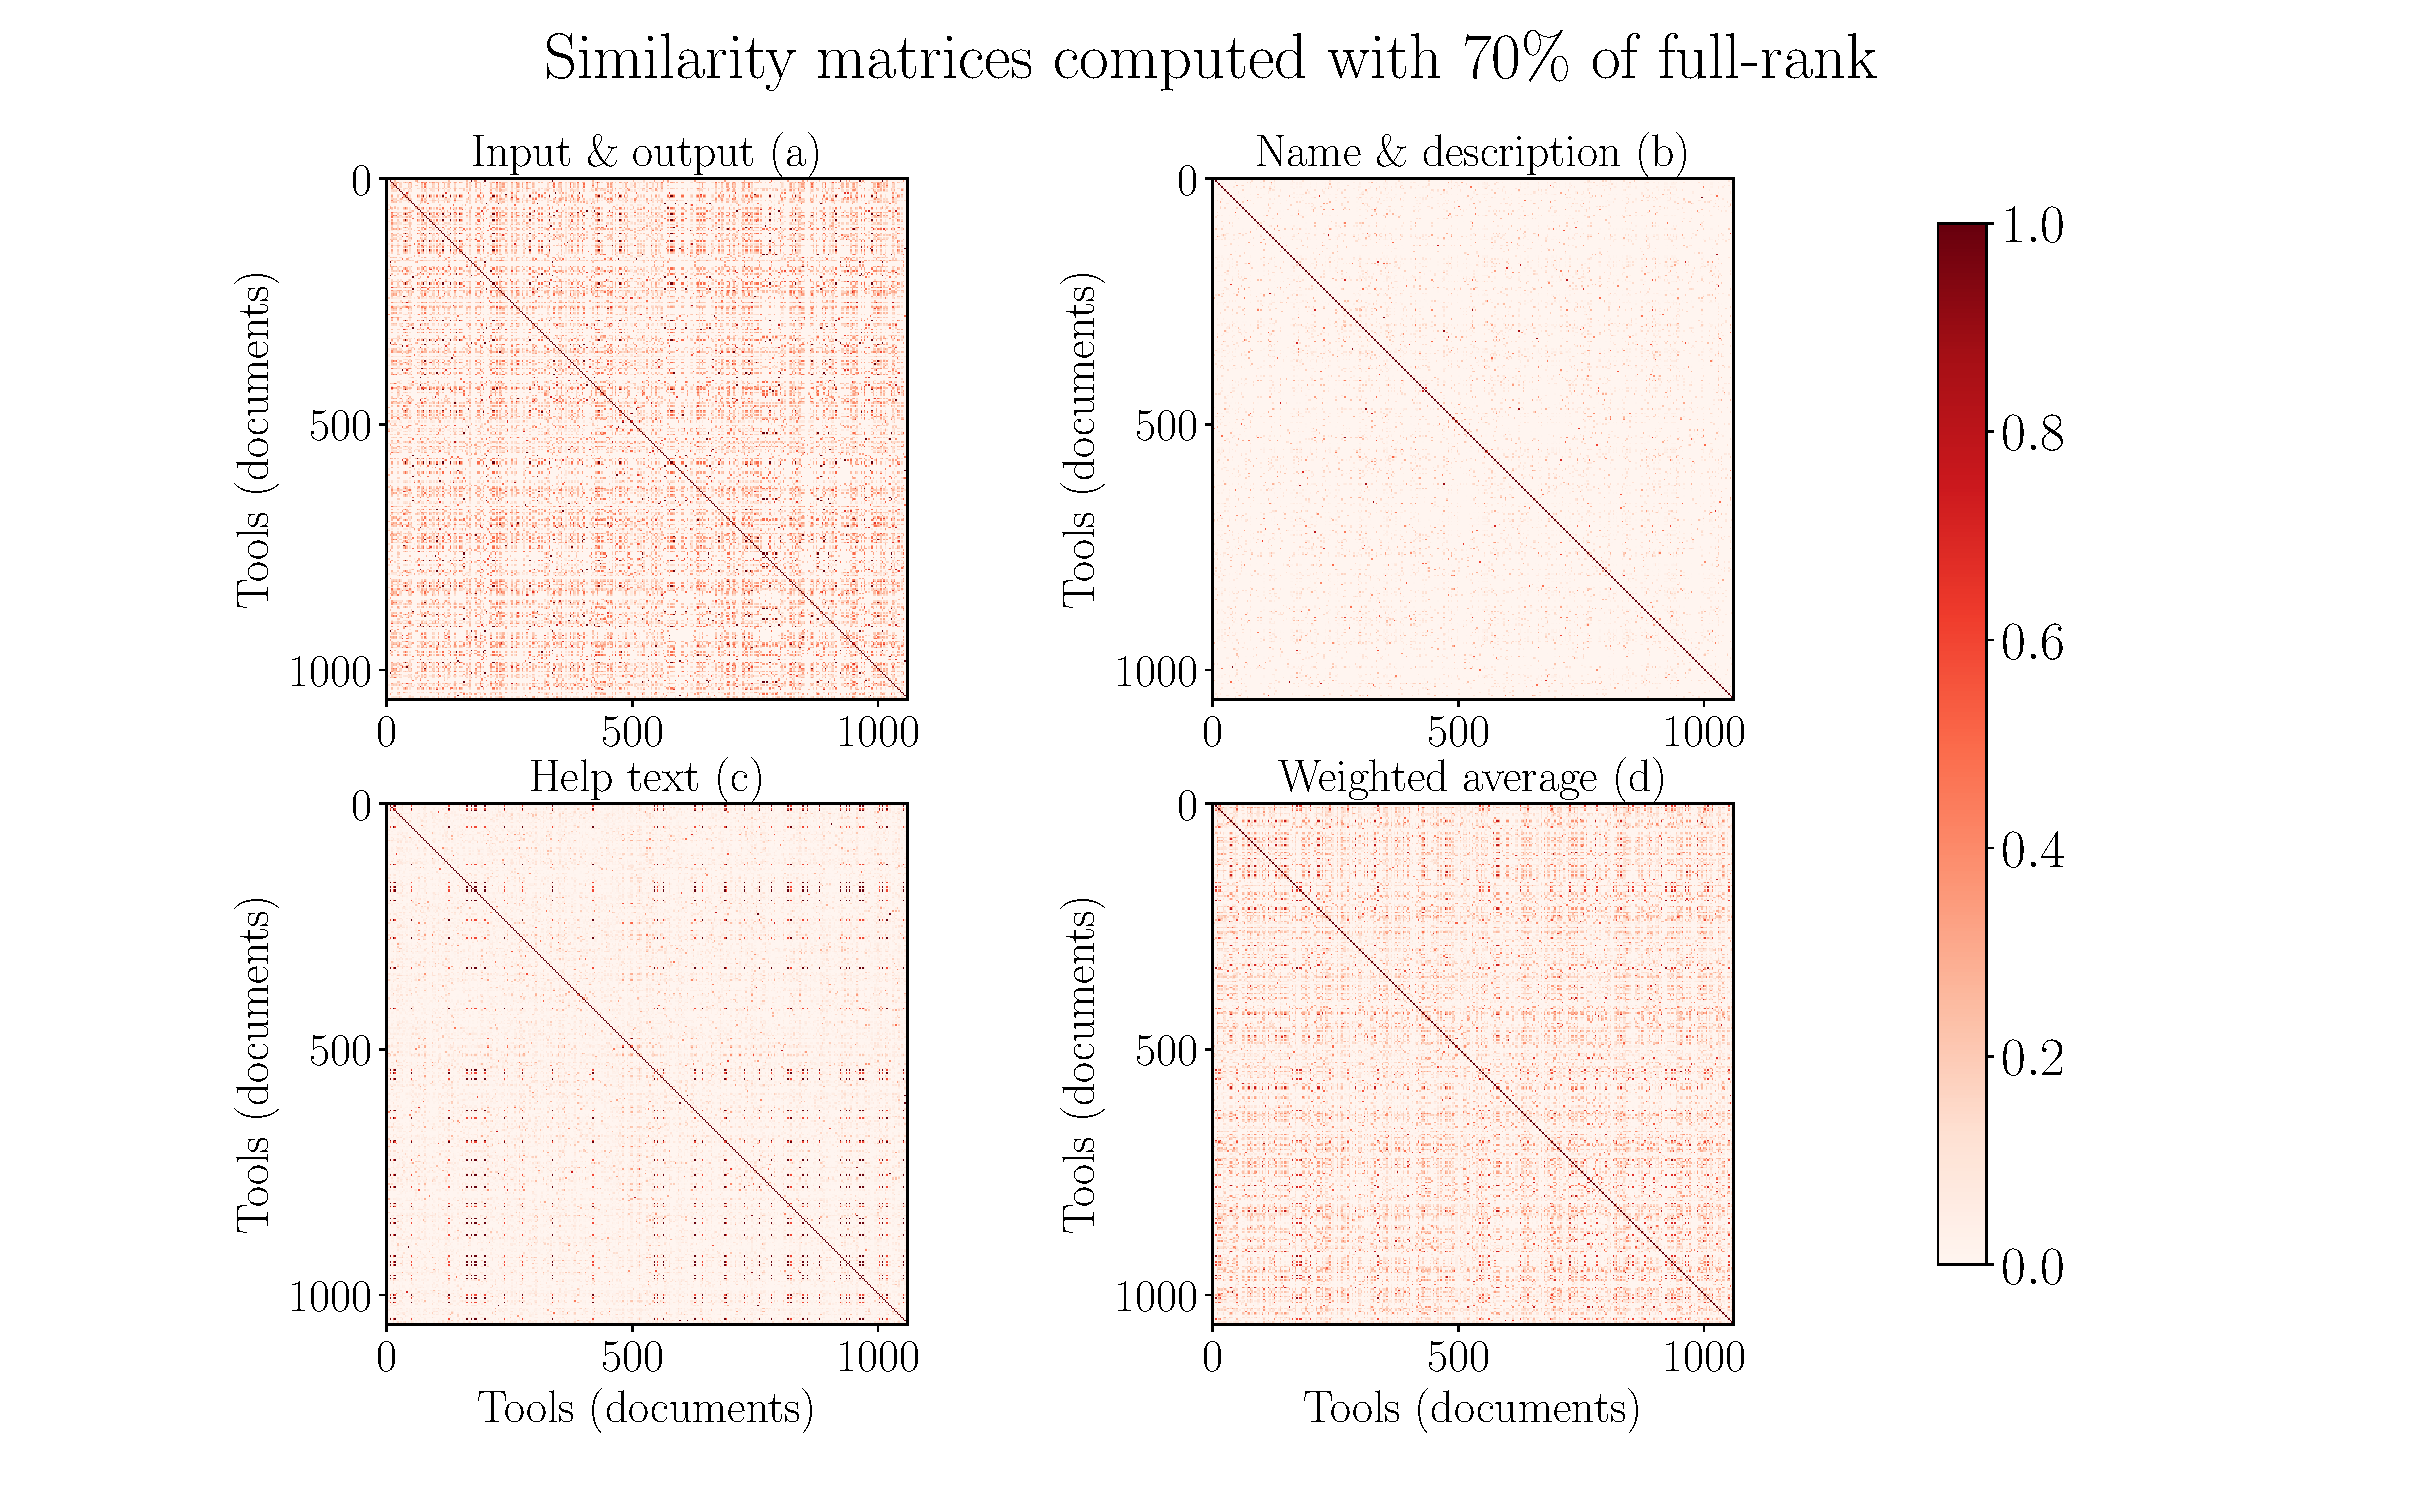
\includegraphics[scale=0.35]{figures/Similarity_matrices_070.pdf}}
    \caption[Similarity matrices 70\% rank]{\textbf{Similarity matrices using 70\% rank}: this correlation plot shows the individual similarity matrices for multiple attributes and the weighted average of these matrices as optimal one after reducing the name and description and help text matrices to 70\% of their respective ranks.}
\end{centering}
\end{figure}

\begin{figure}[h]
\begin{centering}
    {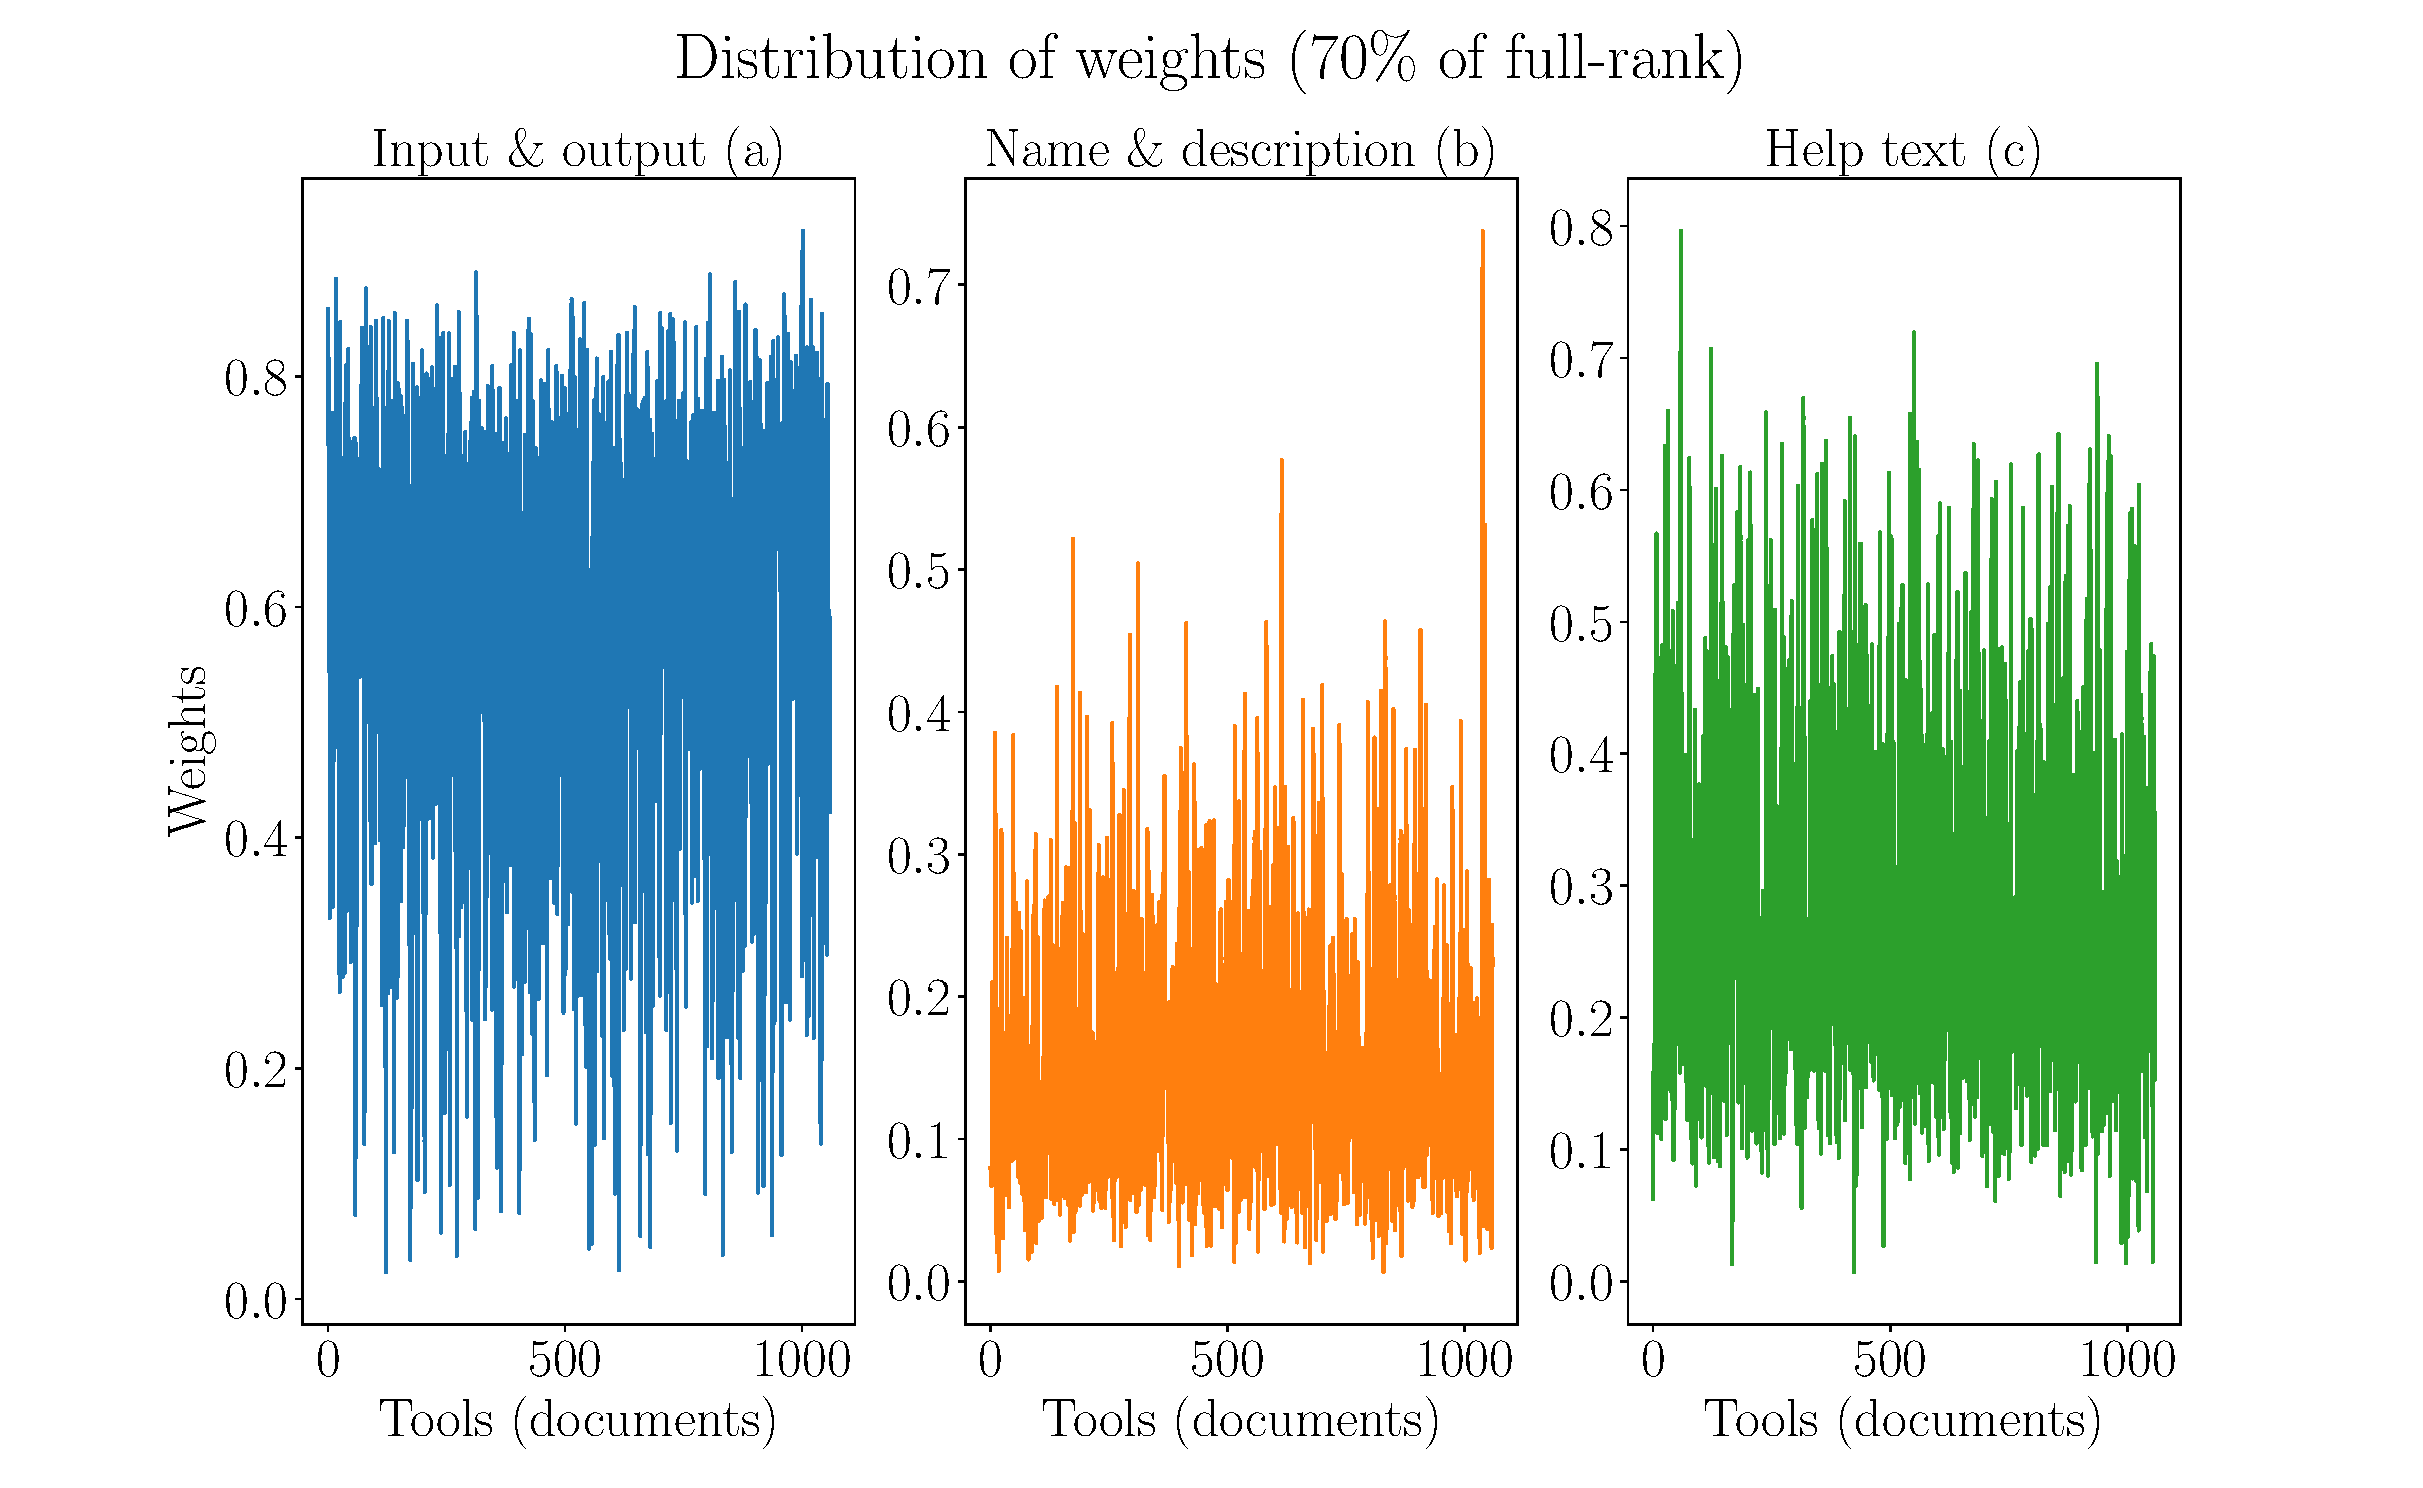
\includegraphics[scale=0.35]{figures/Weights_070.pdf}}
    \caption[Weights distribution 70\% rank]{\textbf{Weights distribution using 70\% rank}: this plot show how the weights vary for multiple tool attributes after reducing the name and description and help text matrices to 70\% of their respective ranks.}
\end{centering}
\end{figure}


\subsection{30\% of full-rank}
We reduce the ranks of two documents-tokens matrices to 30\% of the original ranks.

\begin{figure}[h]
\begin{centering}
    {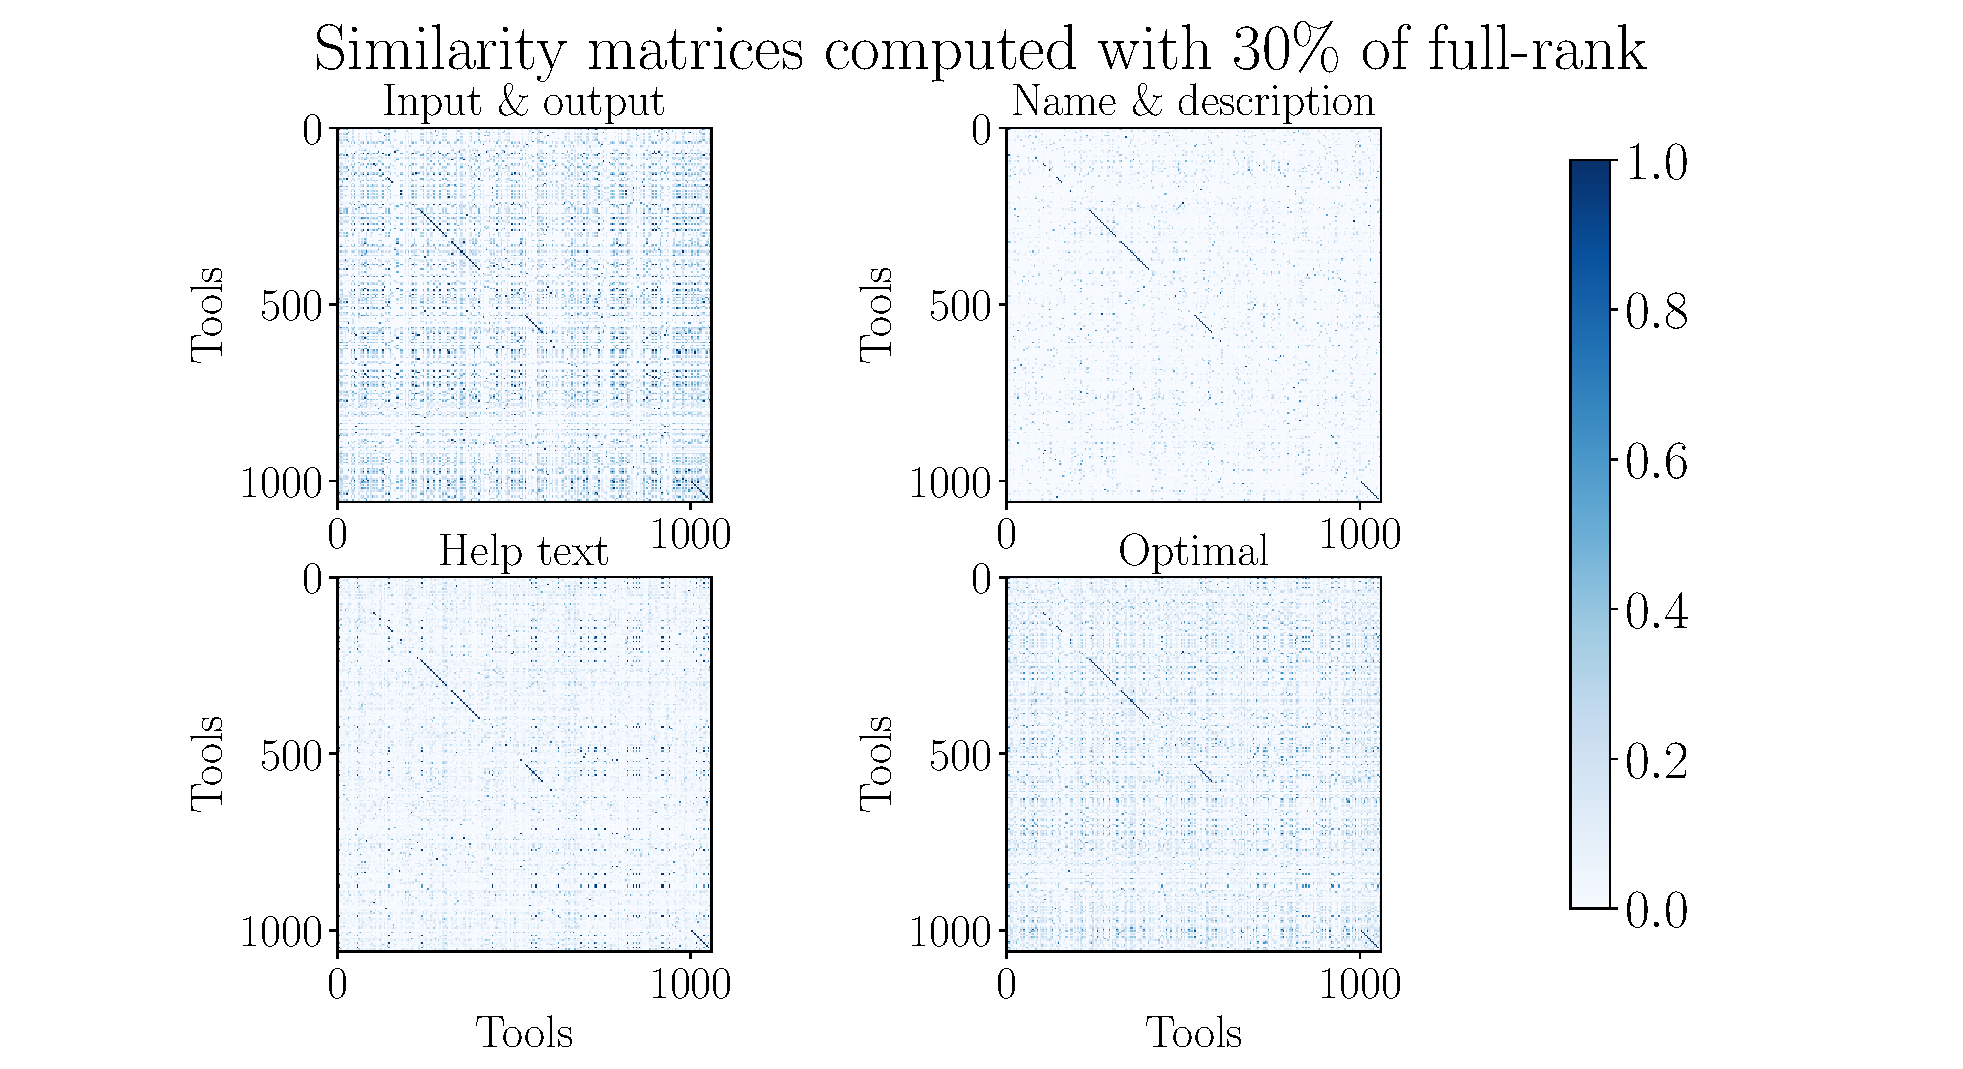
\includegraphics[scale=0.35]{figures/Similarity_matrices_030.pdf}}
    \caption[Similarity matrices 30\% rank]{\textbf{Similarity matrices using 30\% rank}: this correlation plot shows the individual similarity matrices for multiple attributes and the weighted average of these matrices as optimal one after reducing the name and description and help text matrices to 30\% of their respective ranks.}
\end{centering}
\end{figure}

\begin{figure}[h]
\begin{centering}
    {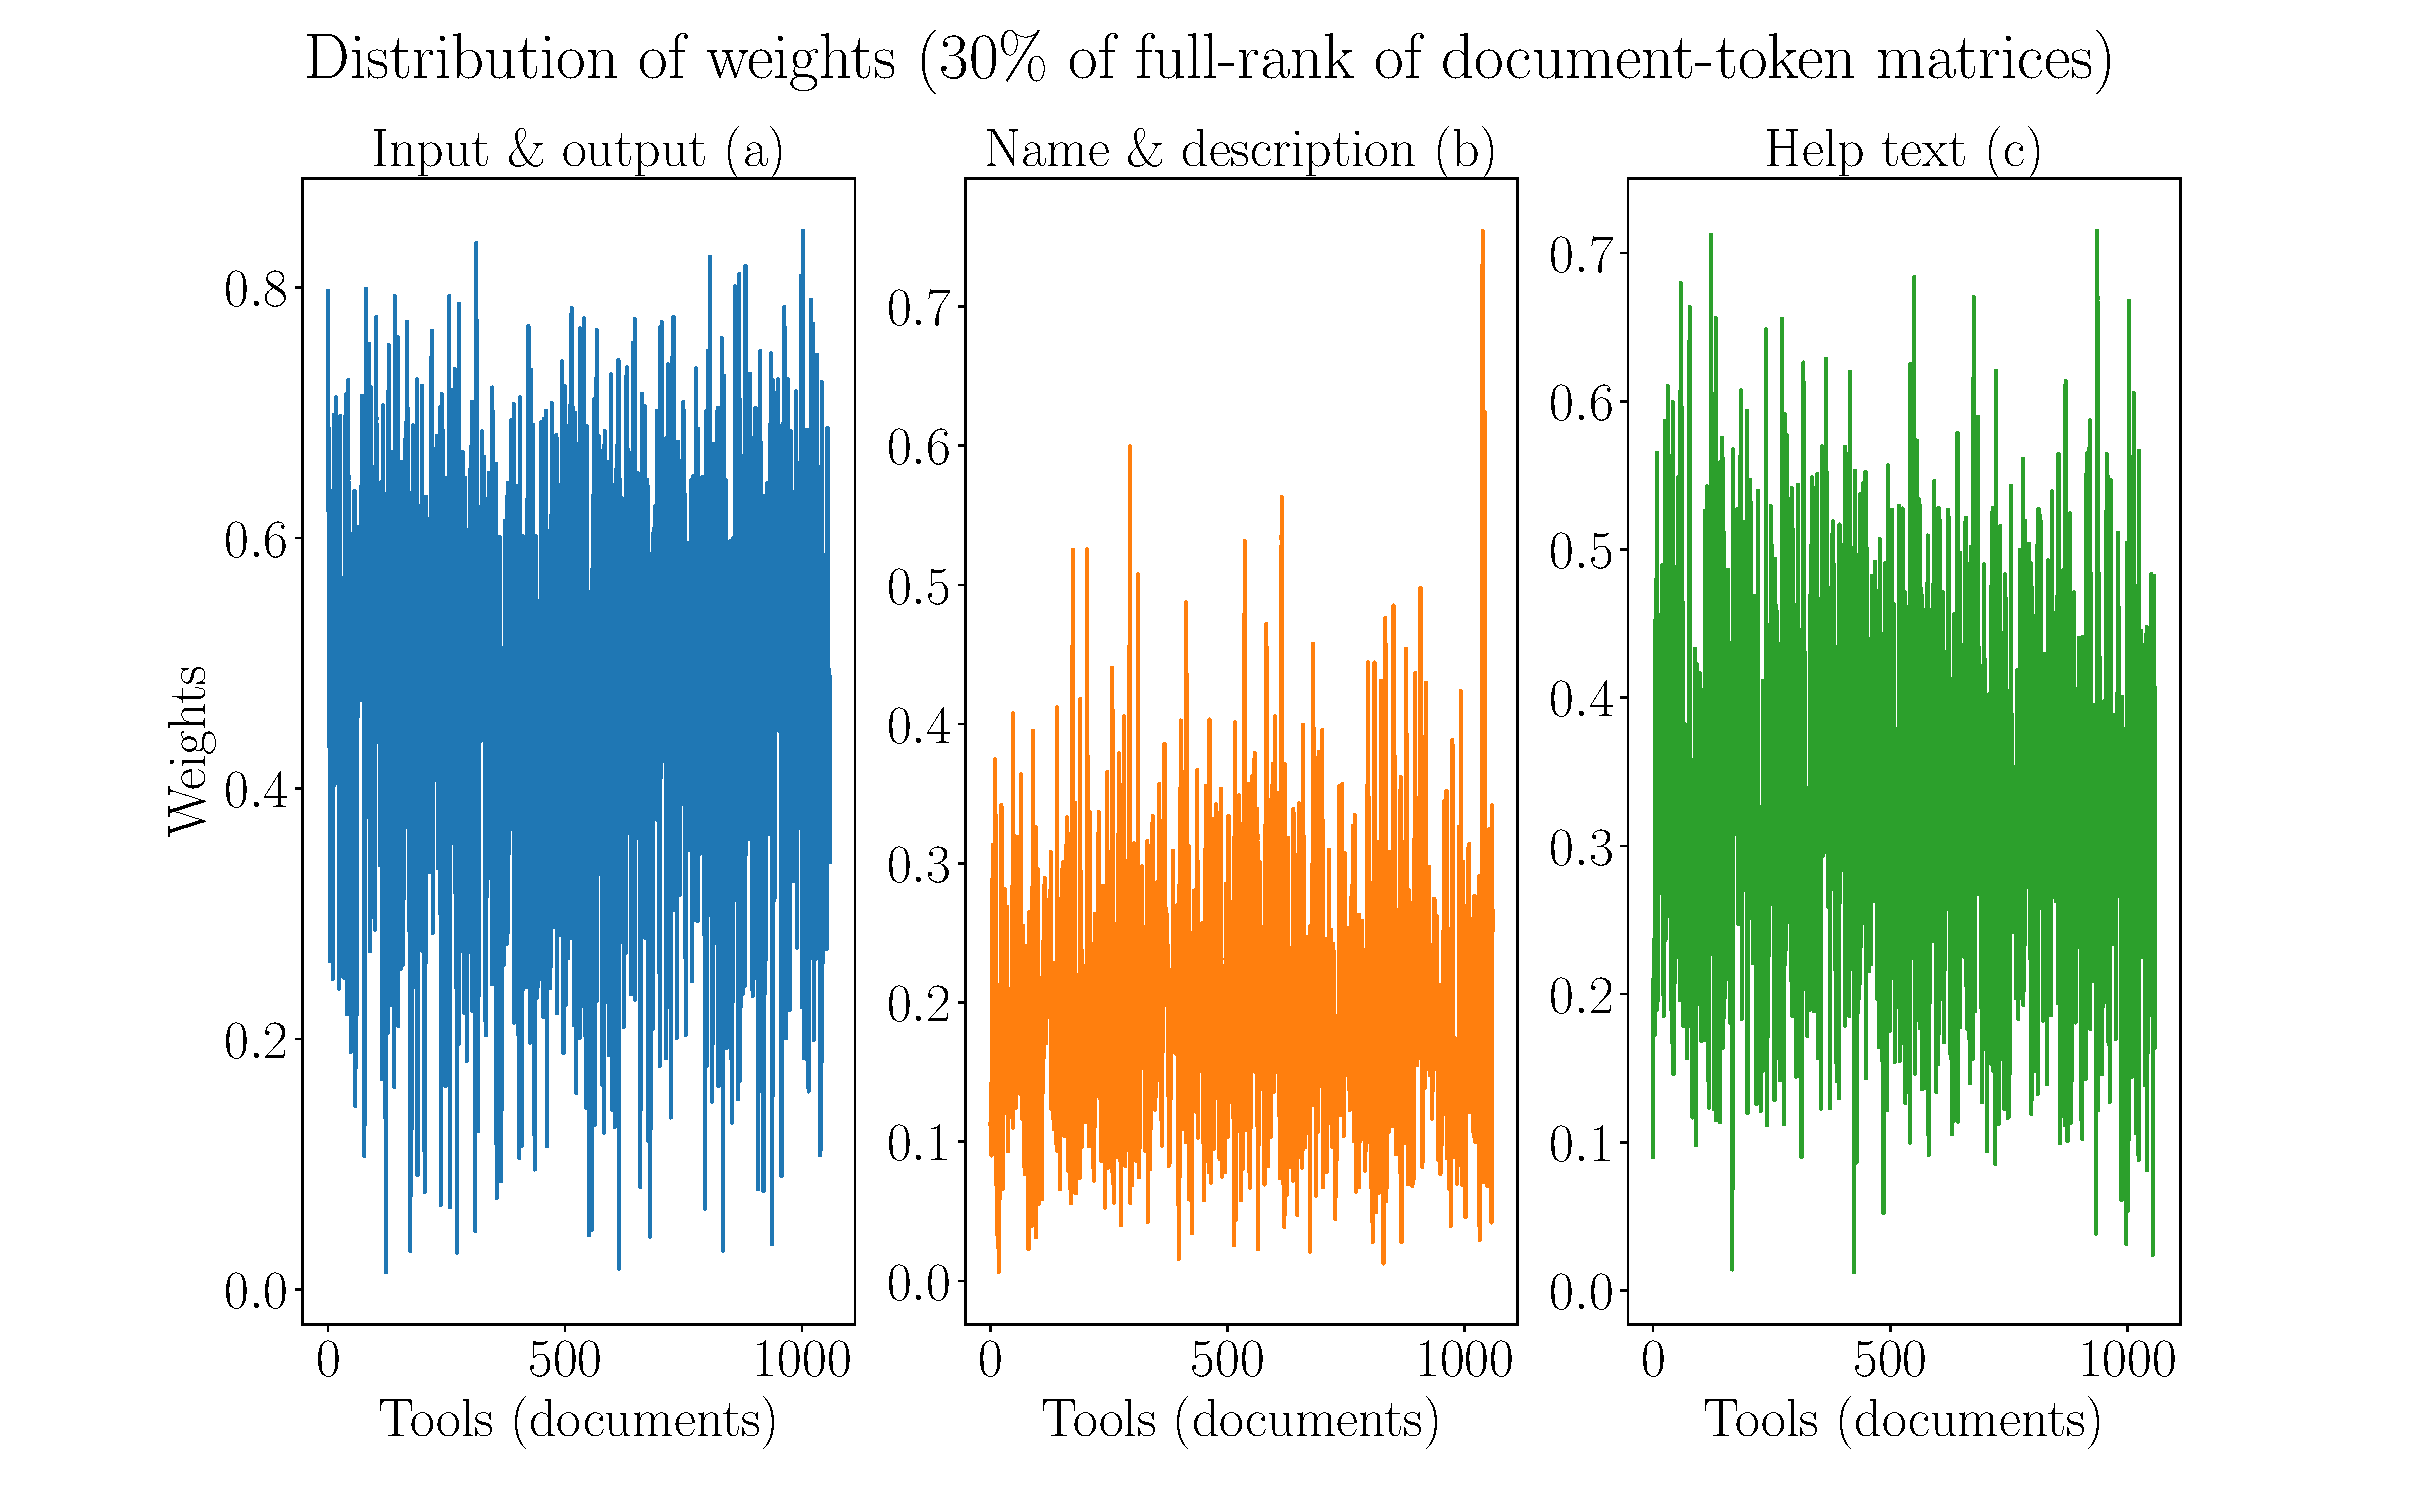
\includegraphics[scale=0.35]{figures/Weights_030.pdf}}
    \caption[Weights distribution 30\% rank]{\textbf{Weights distribution using 30\% rank}: this plot show how the weights vary for multiple tool attributes after reducing the name and description and help text matrices to 30\% of their respective ranks.}
\end{centering}
\end{figure}

\subsection{5\% of full-rank}
We reduce the ranks of two documents-tokens matrices to 5\% of the original ranks.

\begin{figure}[h]
\begin{centering}
    {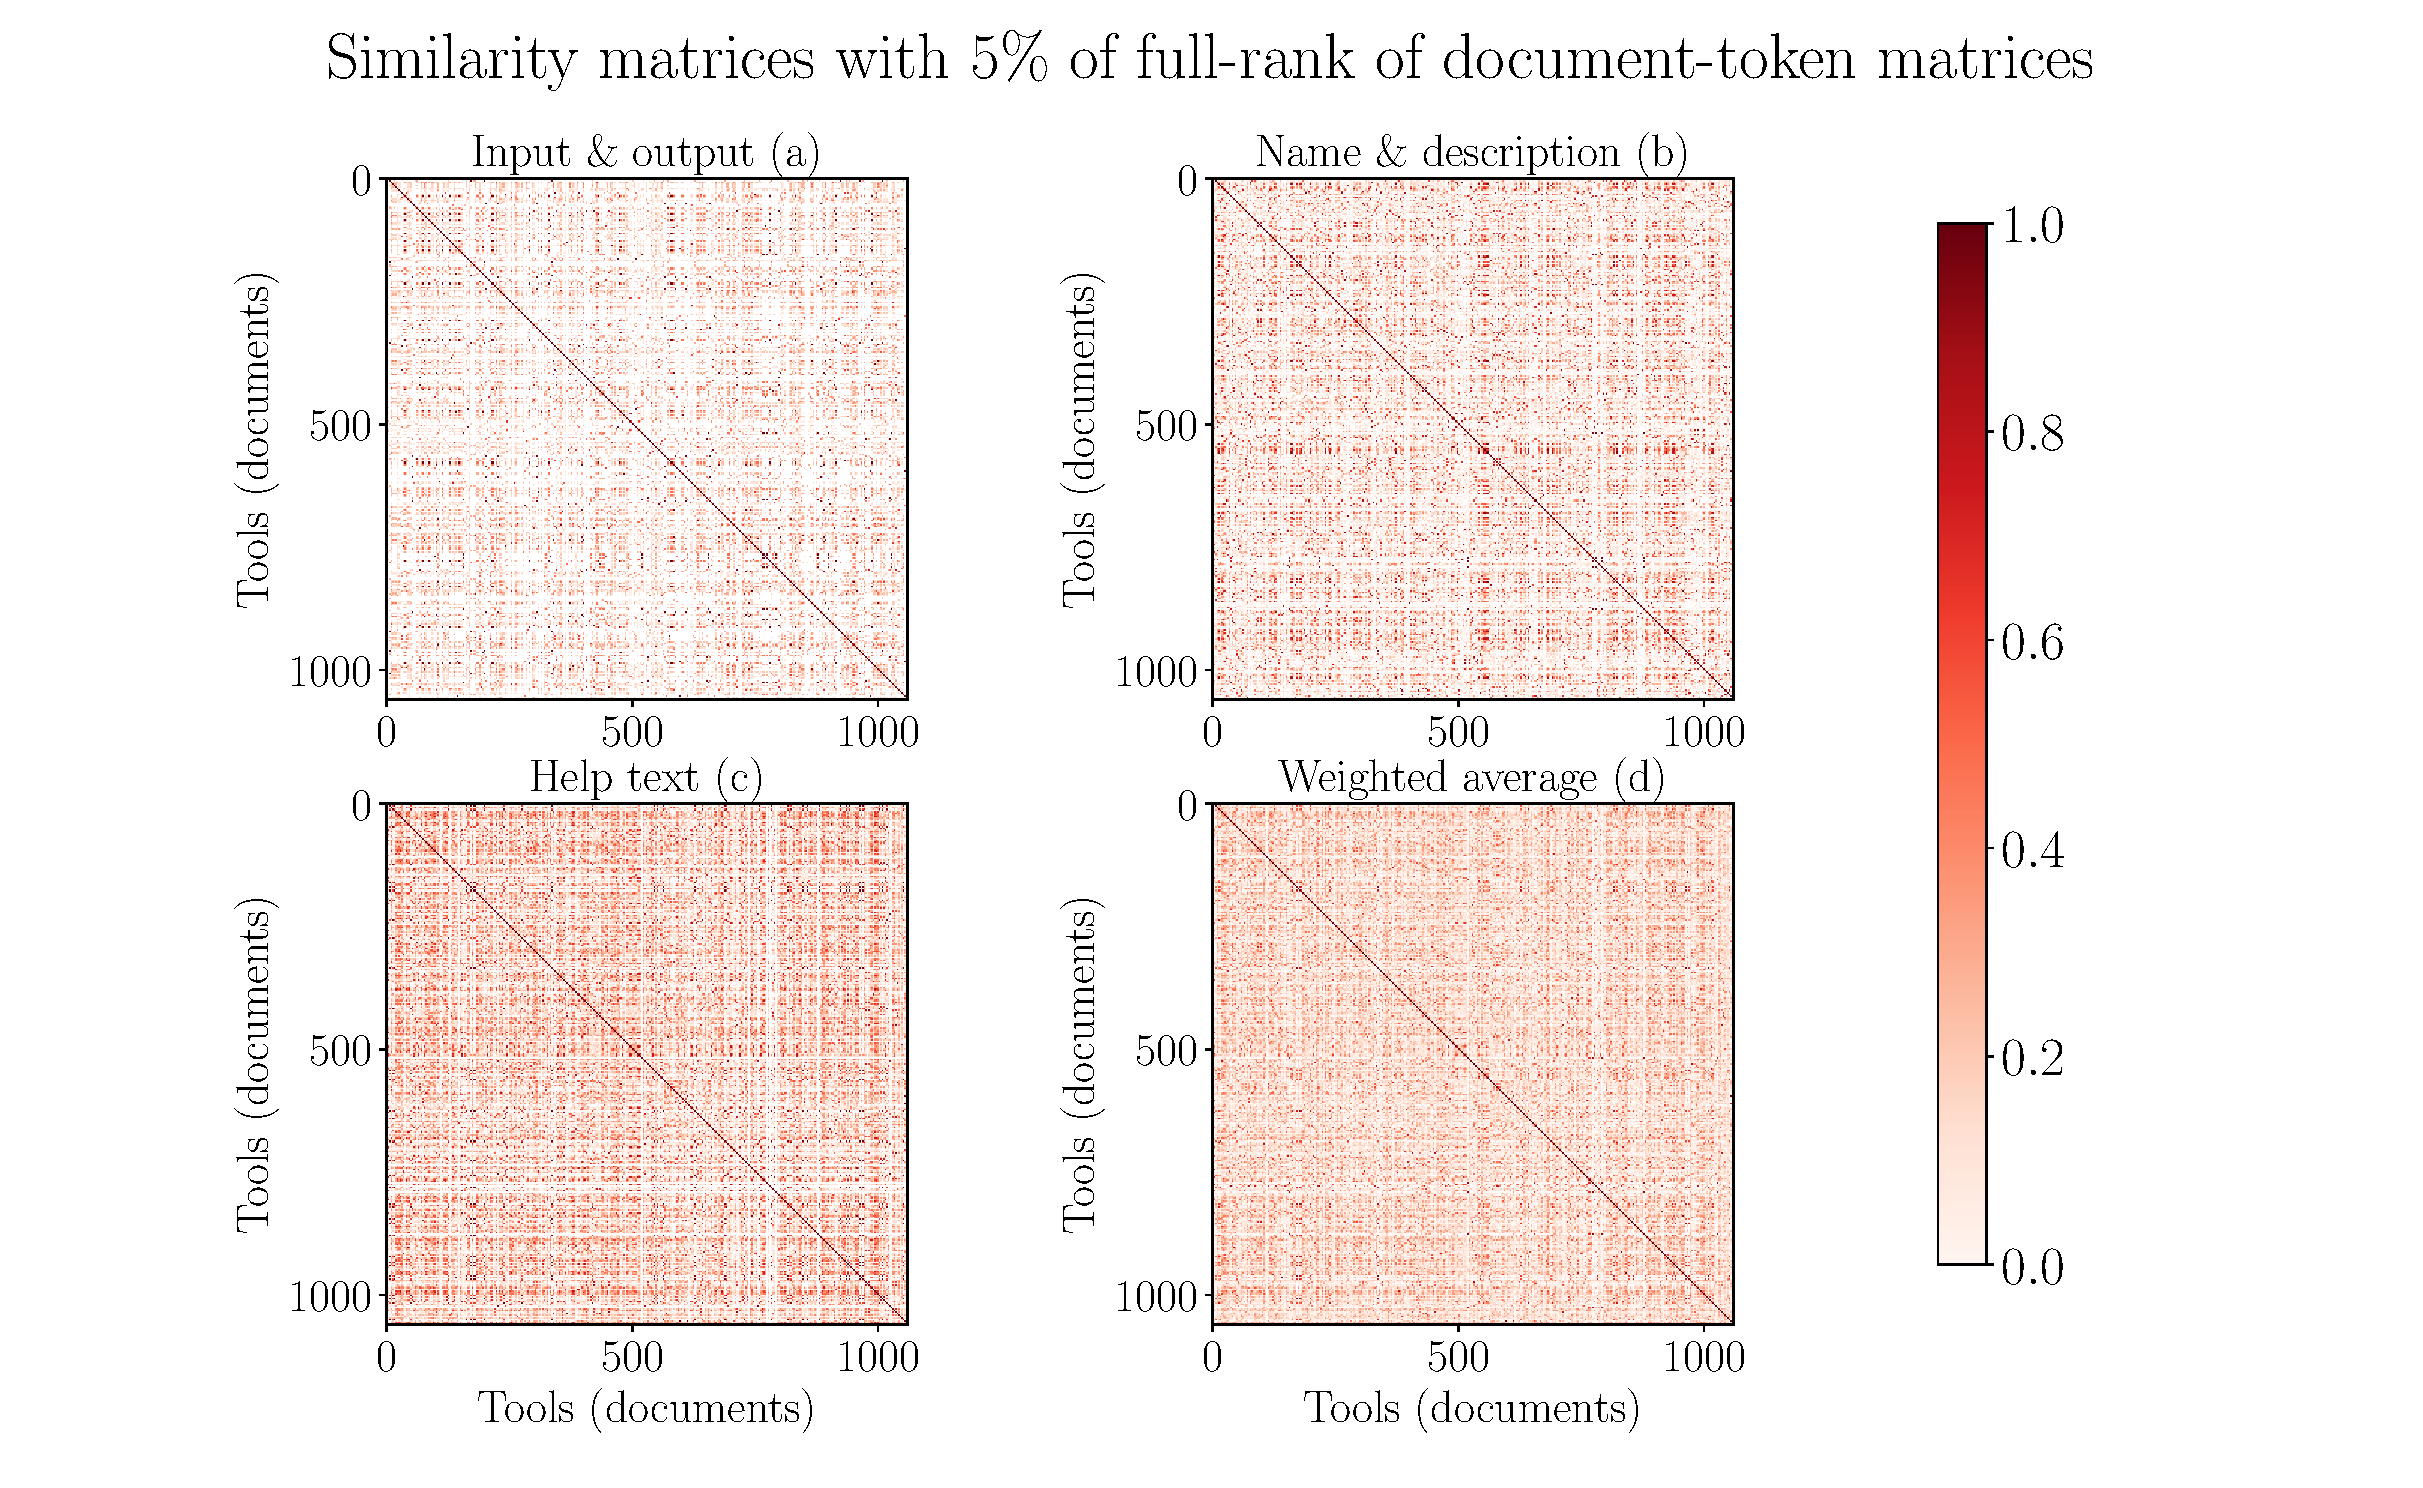
\includegraphics[scale=0.35]{figures/Similarity_matrices_005.pdf}}
    \caption[Similarity matrices 5\% rank]{\textbf{Similarity matrices using 5\% rank}: this correlation plot shows the individual similarity matrices for multiple attributes and the weighted average of these matrices as optimal one after reducing the name and description and help text matrices to 5\% of their respective ranks.}
\end{centering}
\end{figure}

\begin{figure}[h]
\begin{centering}
    {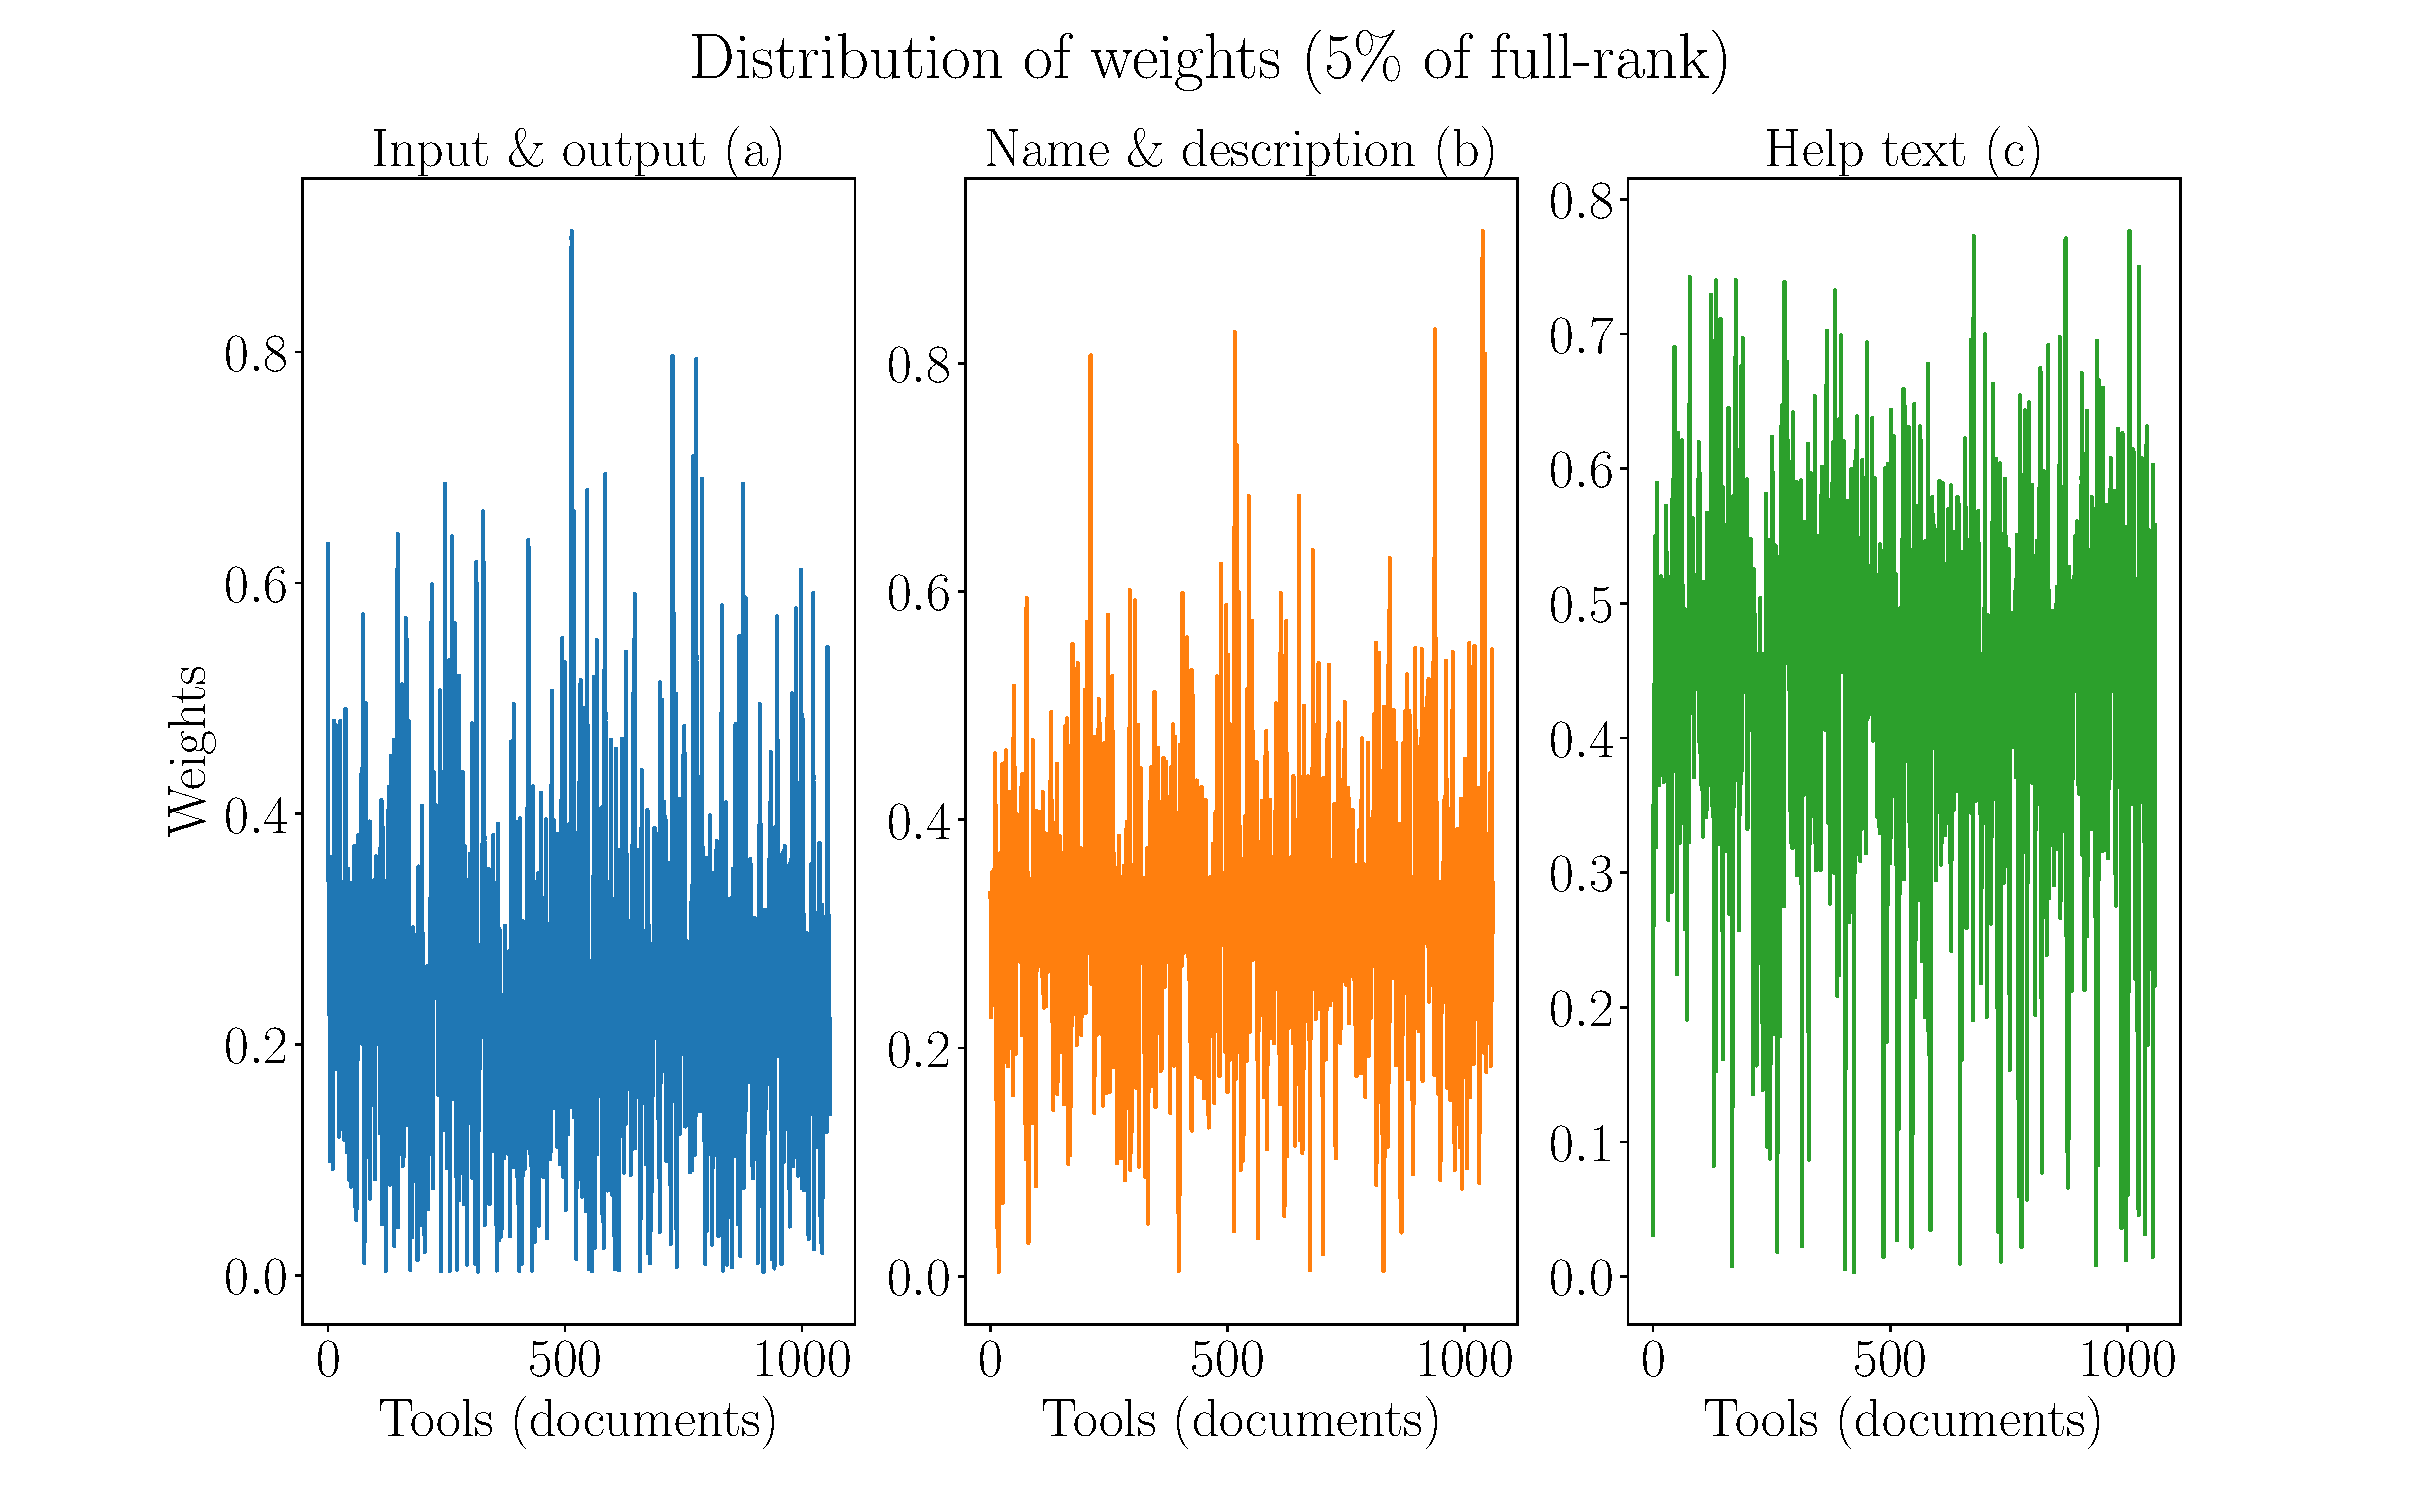
\includegraphics[scale=0.35]{figures/Weights_005.pdf}}
    \caption[Weights distribution 5\% rank]{\textbf{Weights distribution using 5\% rank}: this plot show how the weights vary for multiple tool attributes after reducing the name and description and help text matrices to 5\% of their respective ranks.}
\end{centering}
\end{figure}

\subsection{Reduction in error}
We observe the loss in mean squared error when we decrease the ranks of the matrices. When we reduced the ranks, the similarity scores for the name and description and help text increase. This increase accounts for their higher importance weights learnt by the optimizer. The importance weights on an average become more balanced and can account for the decrease in the mean squared error. We would also see that in the next section that the ranking of similar tools also become better after rank reduction.

\begin{figure}[h]
\begin{centering}
    {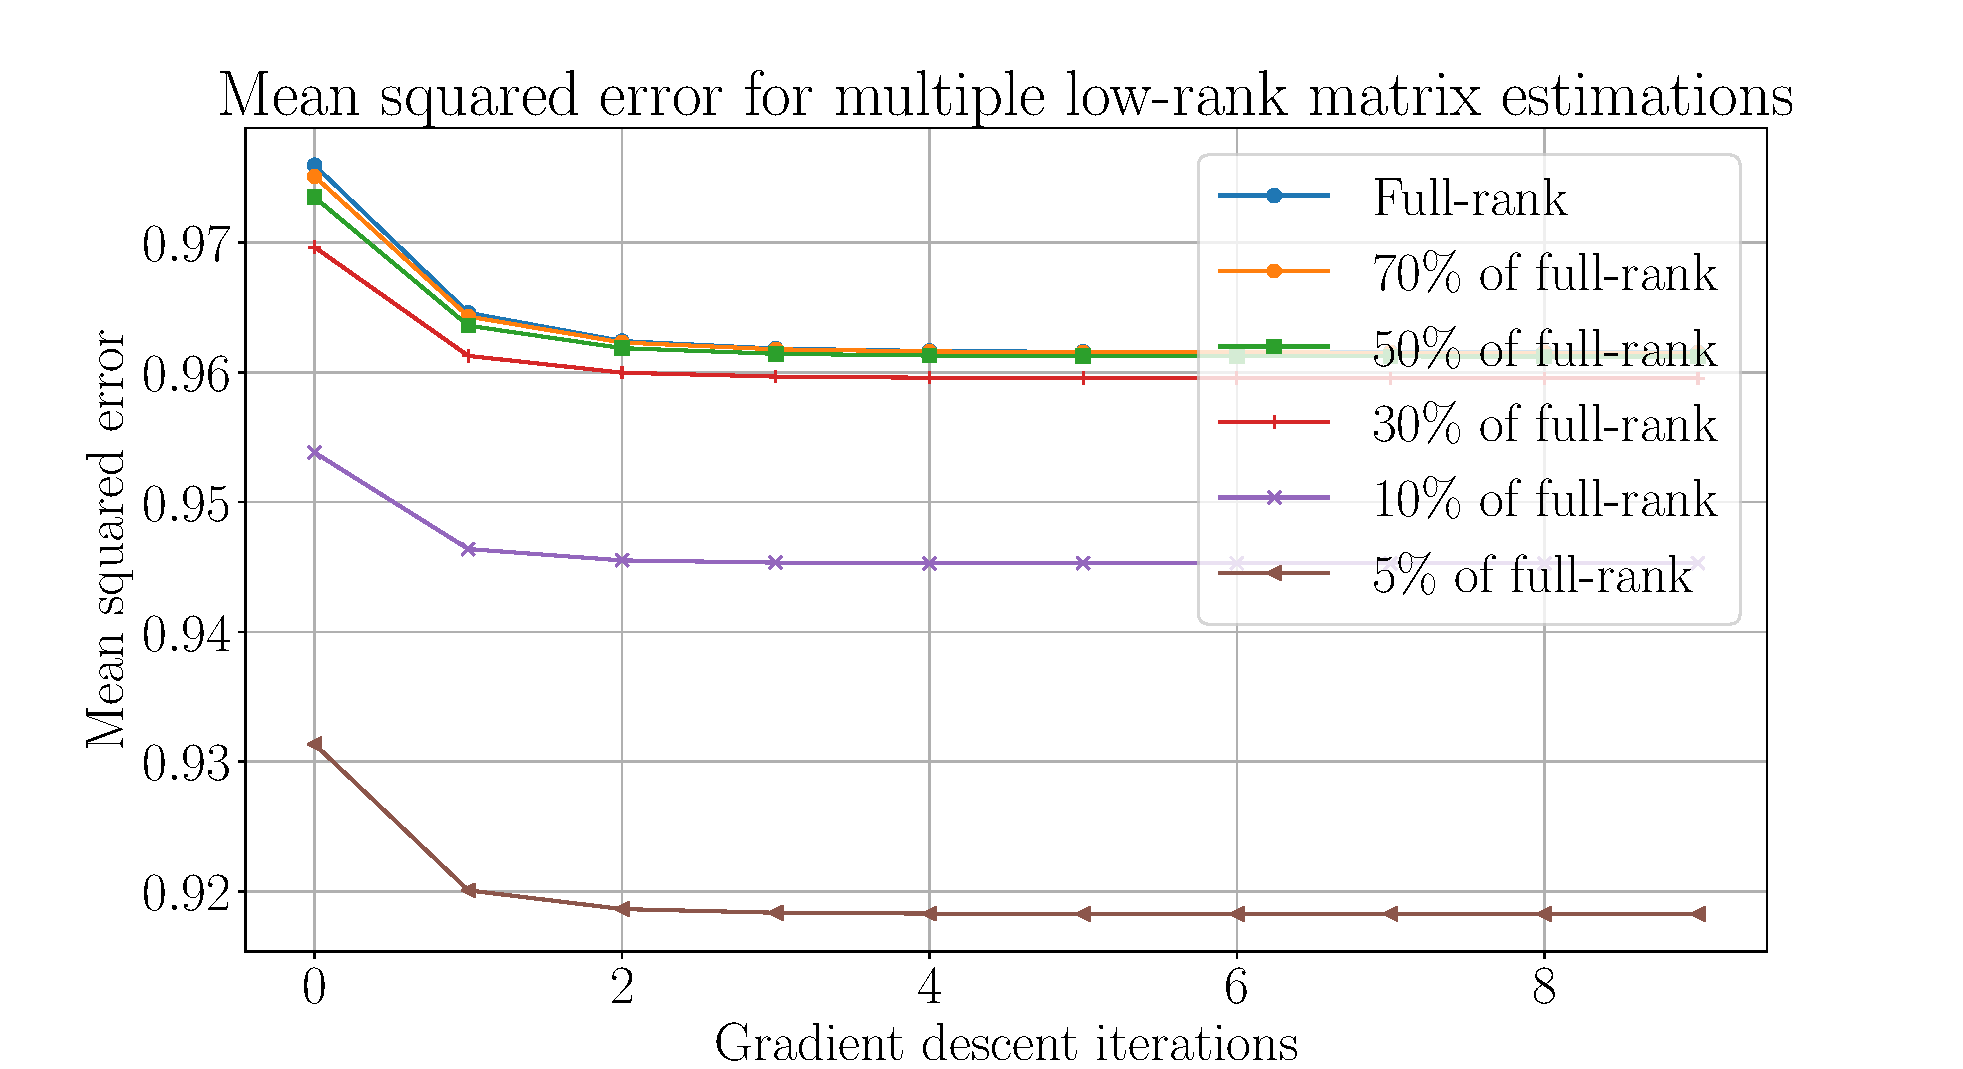
\includegraphics[scale=0.35]{figures/MSE_iterations_low_rank.pdf}}
    \caption[Similarity matrices 5\% rank]{\textbf{Similarity matrices using 5\% rank}: this correlation plot shows the individual similarity matrices for multiple attributes and the weighted average of these matrices as optimal one after reducing the name and description and help text matrices to 5\% of their respective ranks.}
\end{centering}
\end{figure}

\section{Paragraph vectors}

\begin{figure}[h]
\begin{centering}
    {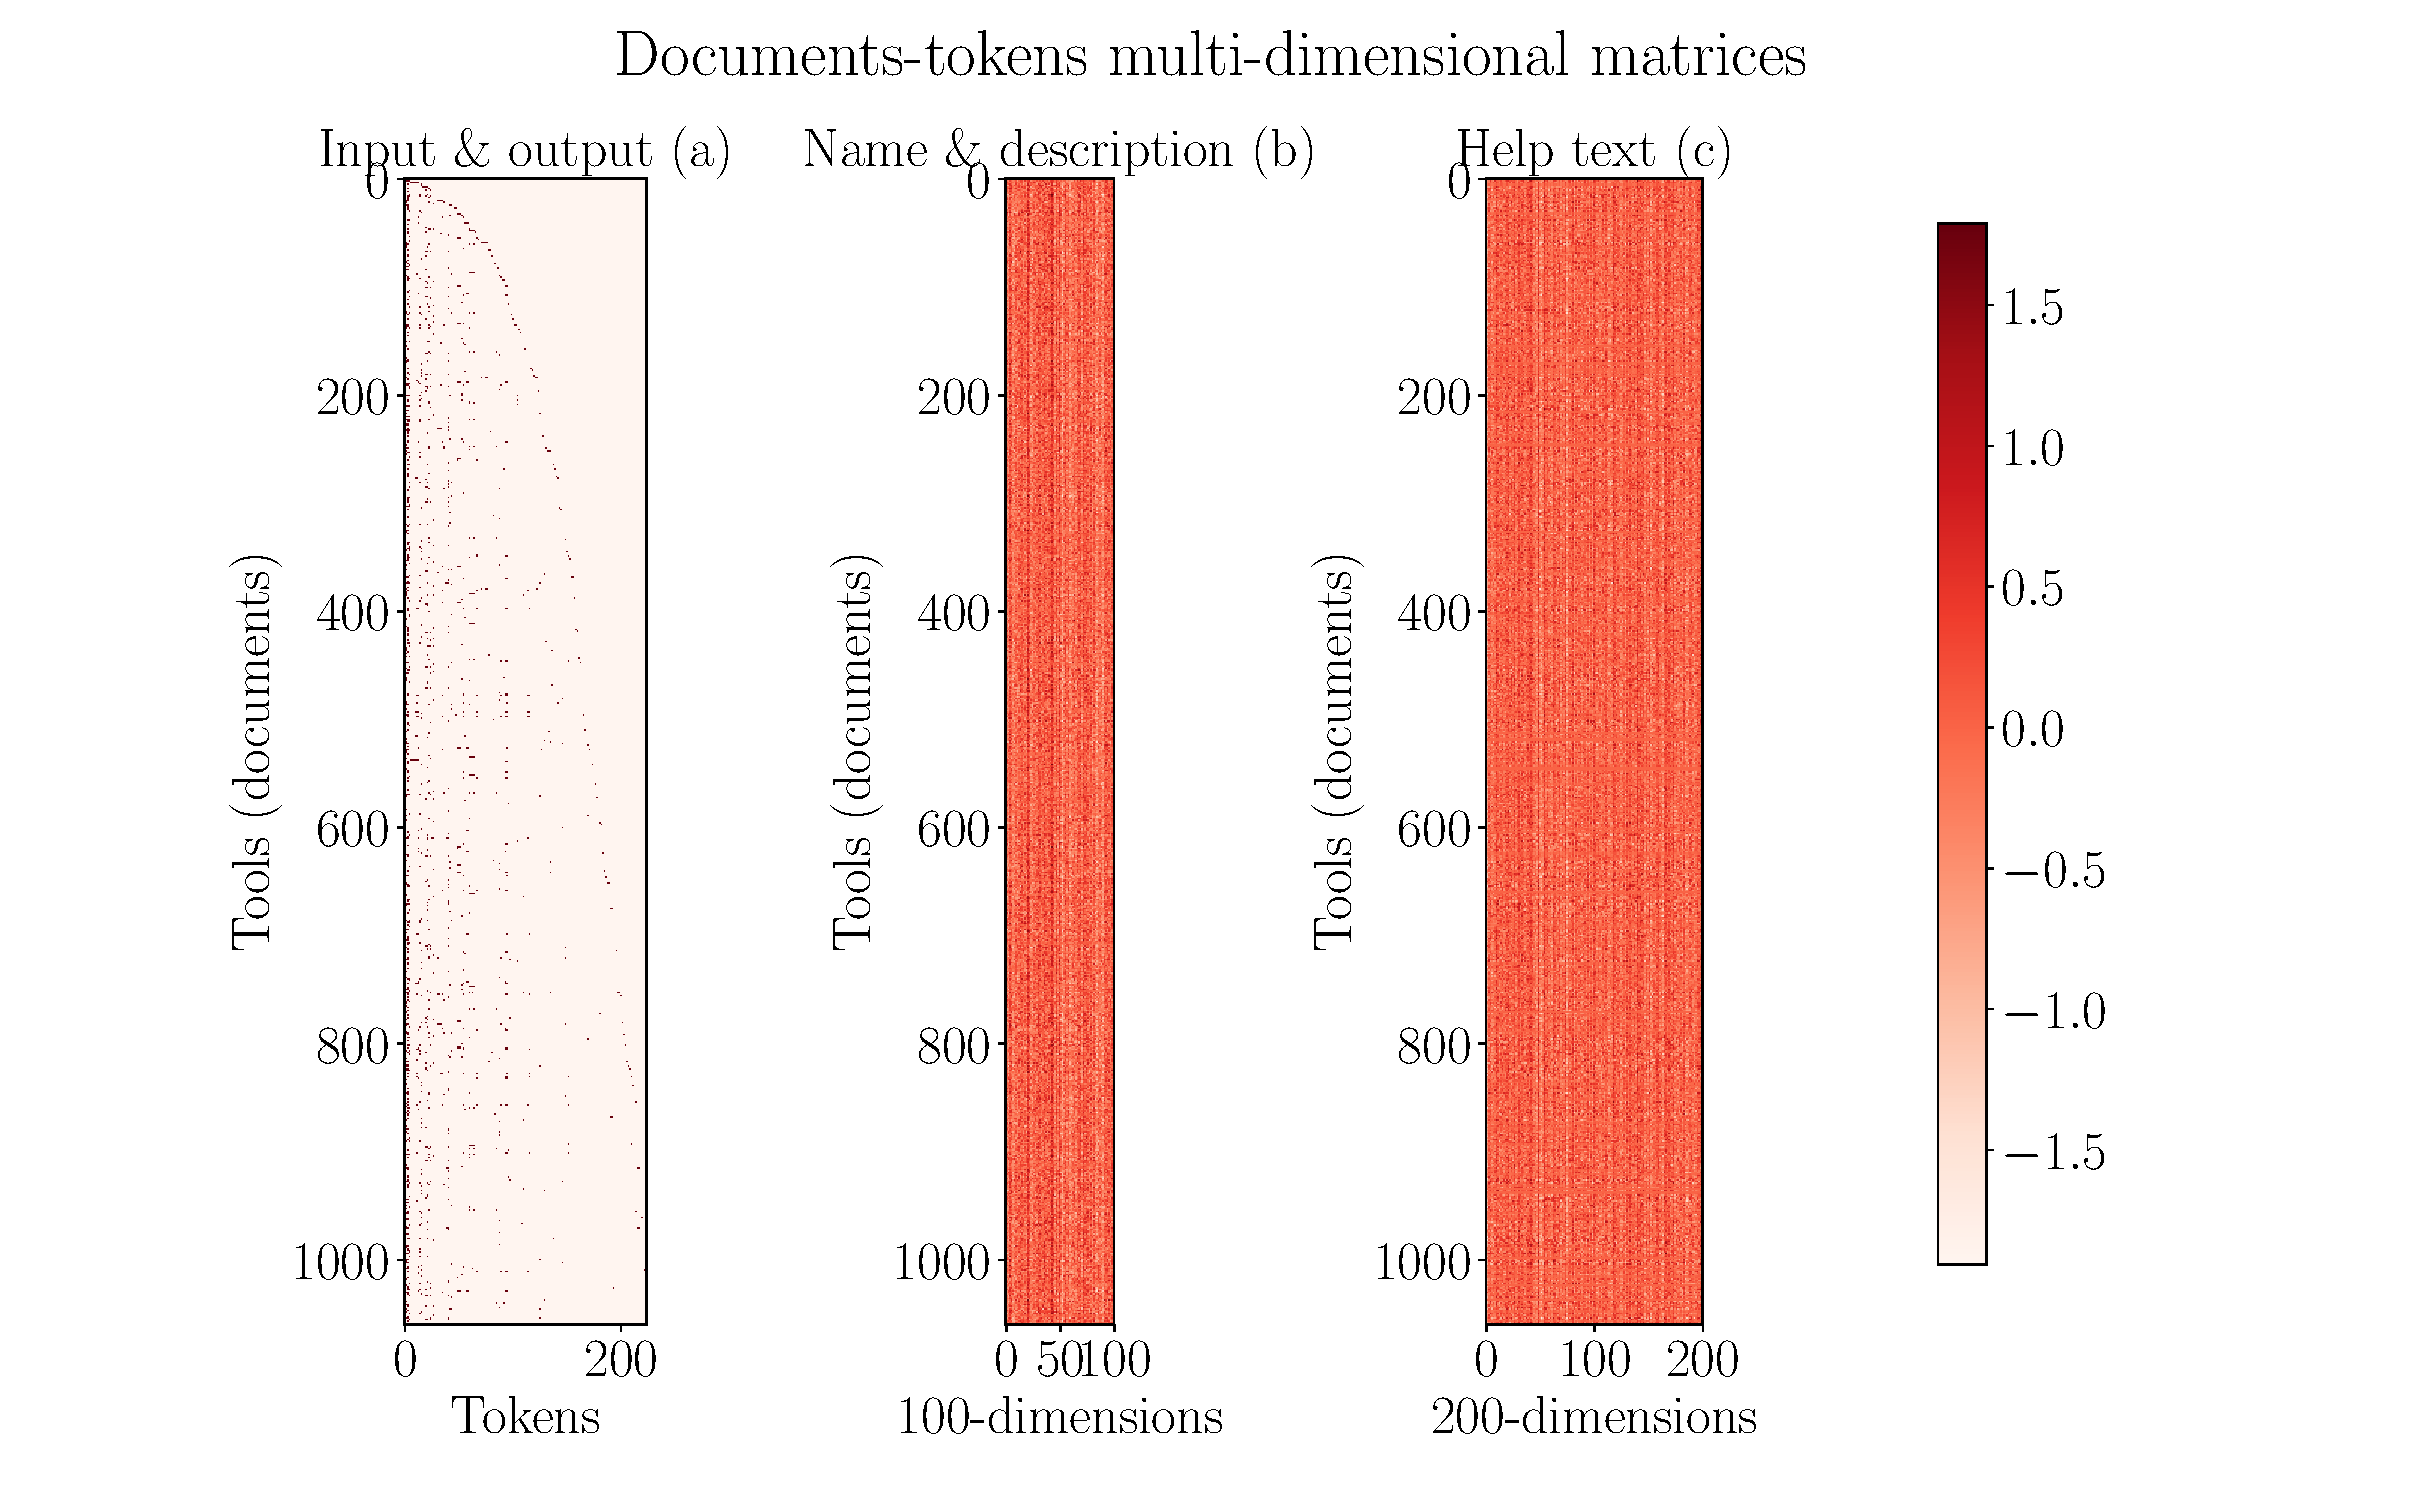
\includegraphics[scale=0.35]{figures/Documents-tokens_doc2vec.pdf}}
    \caption[Documents-tokens matrices for doc2vec]{\textbf{Documents-tokens matrices for Paragraph vectors approach}: this heatmap shows a documents-tokens matrix (the leftmost) for input and output file types. The next two matrices belong to name and description and help text attributes. Each row of both of these matrices is a n-multi-dimensional paragraph vector.}
\end{centering}
\end{figure}


\begin{figure}[h]
\begin{centering}
    {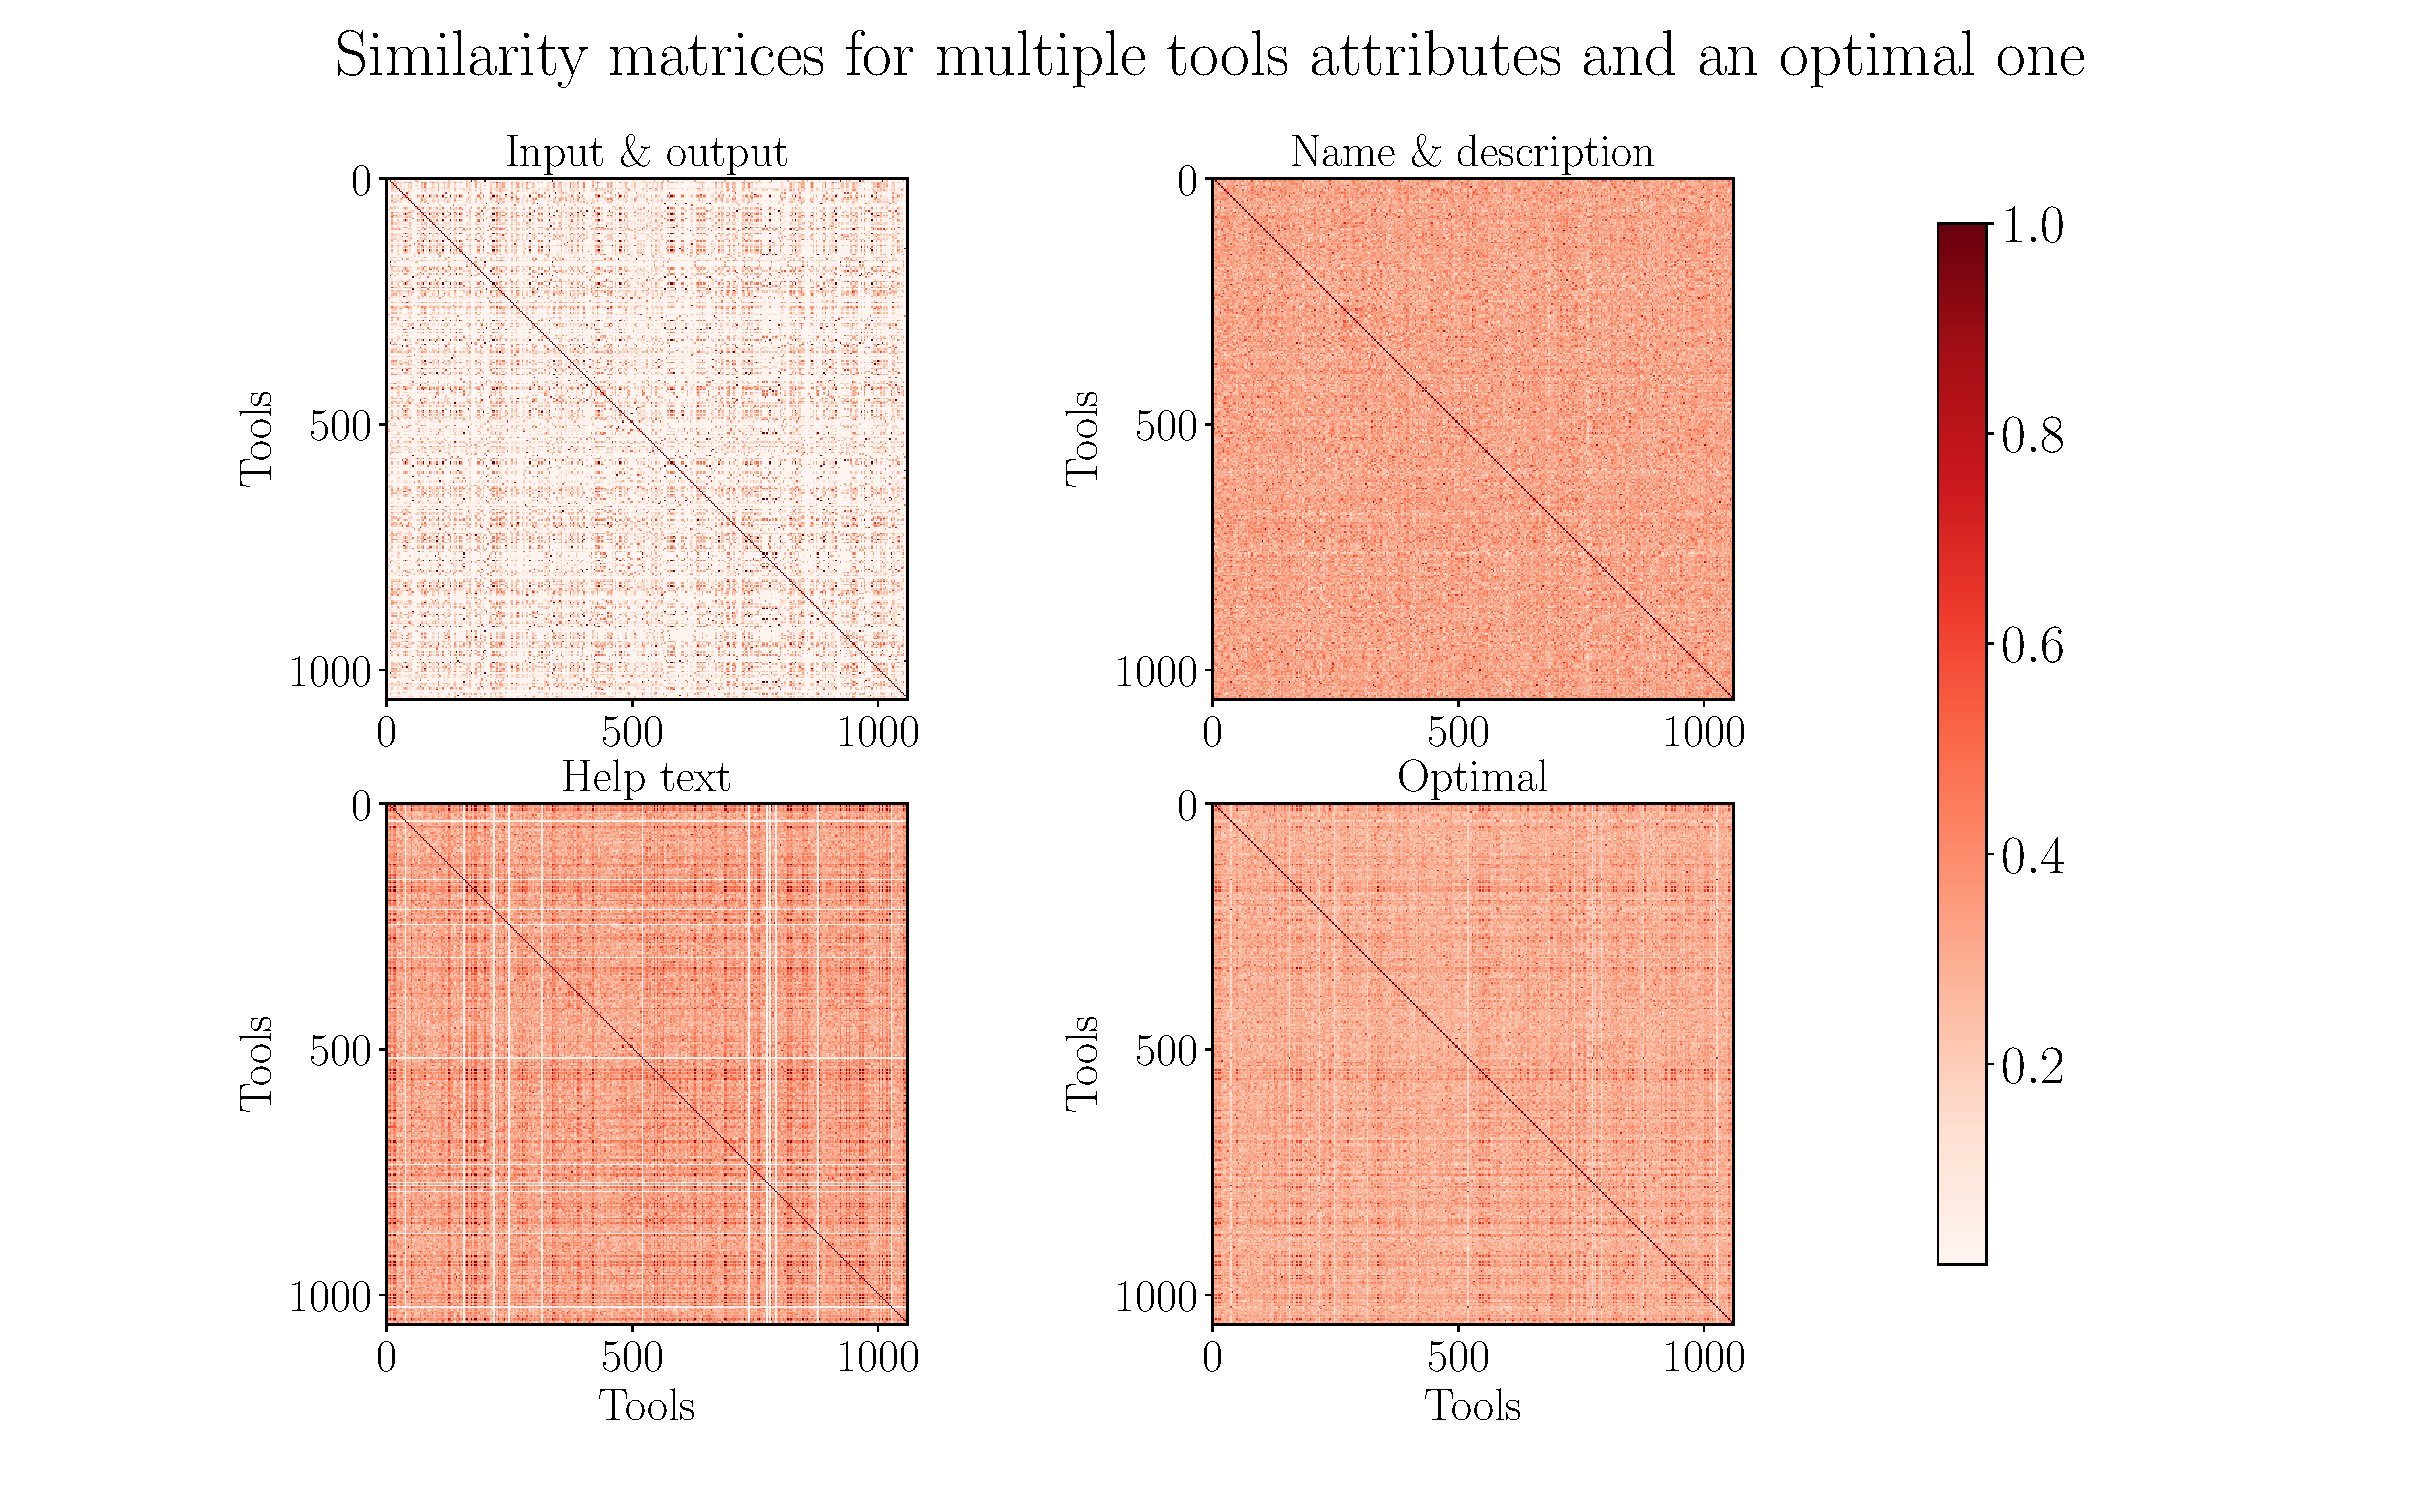
\includegraphics[scale=0.35]{figures/Similarity_matrices_doc2vec.pdf}}
    \caption[Similarity matrices using doc2vec]{\textbf{Similarity matrices computed using "paragraph vectors" approach}: this plot show four correlation heatmaps. The top-left, top-right and bottom-left are the individual correlation matrices for input and output, name and description and help text attributes. The bottom-right one is the weighted average correlation matrix computed from the last three matrices.}
\end{centering}
\end{figure}

\begin{figure}[h]
\begin{centering}
    {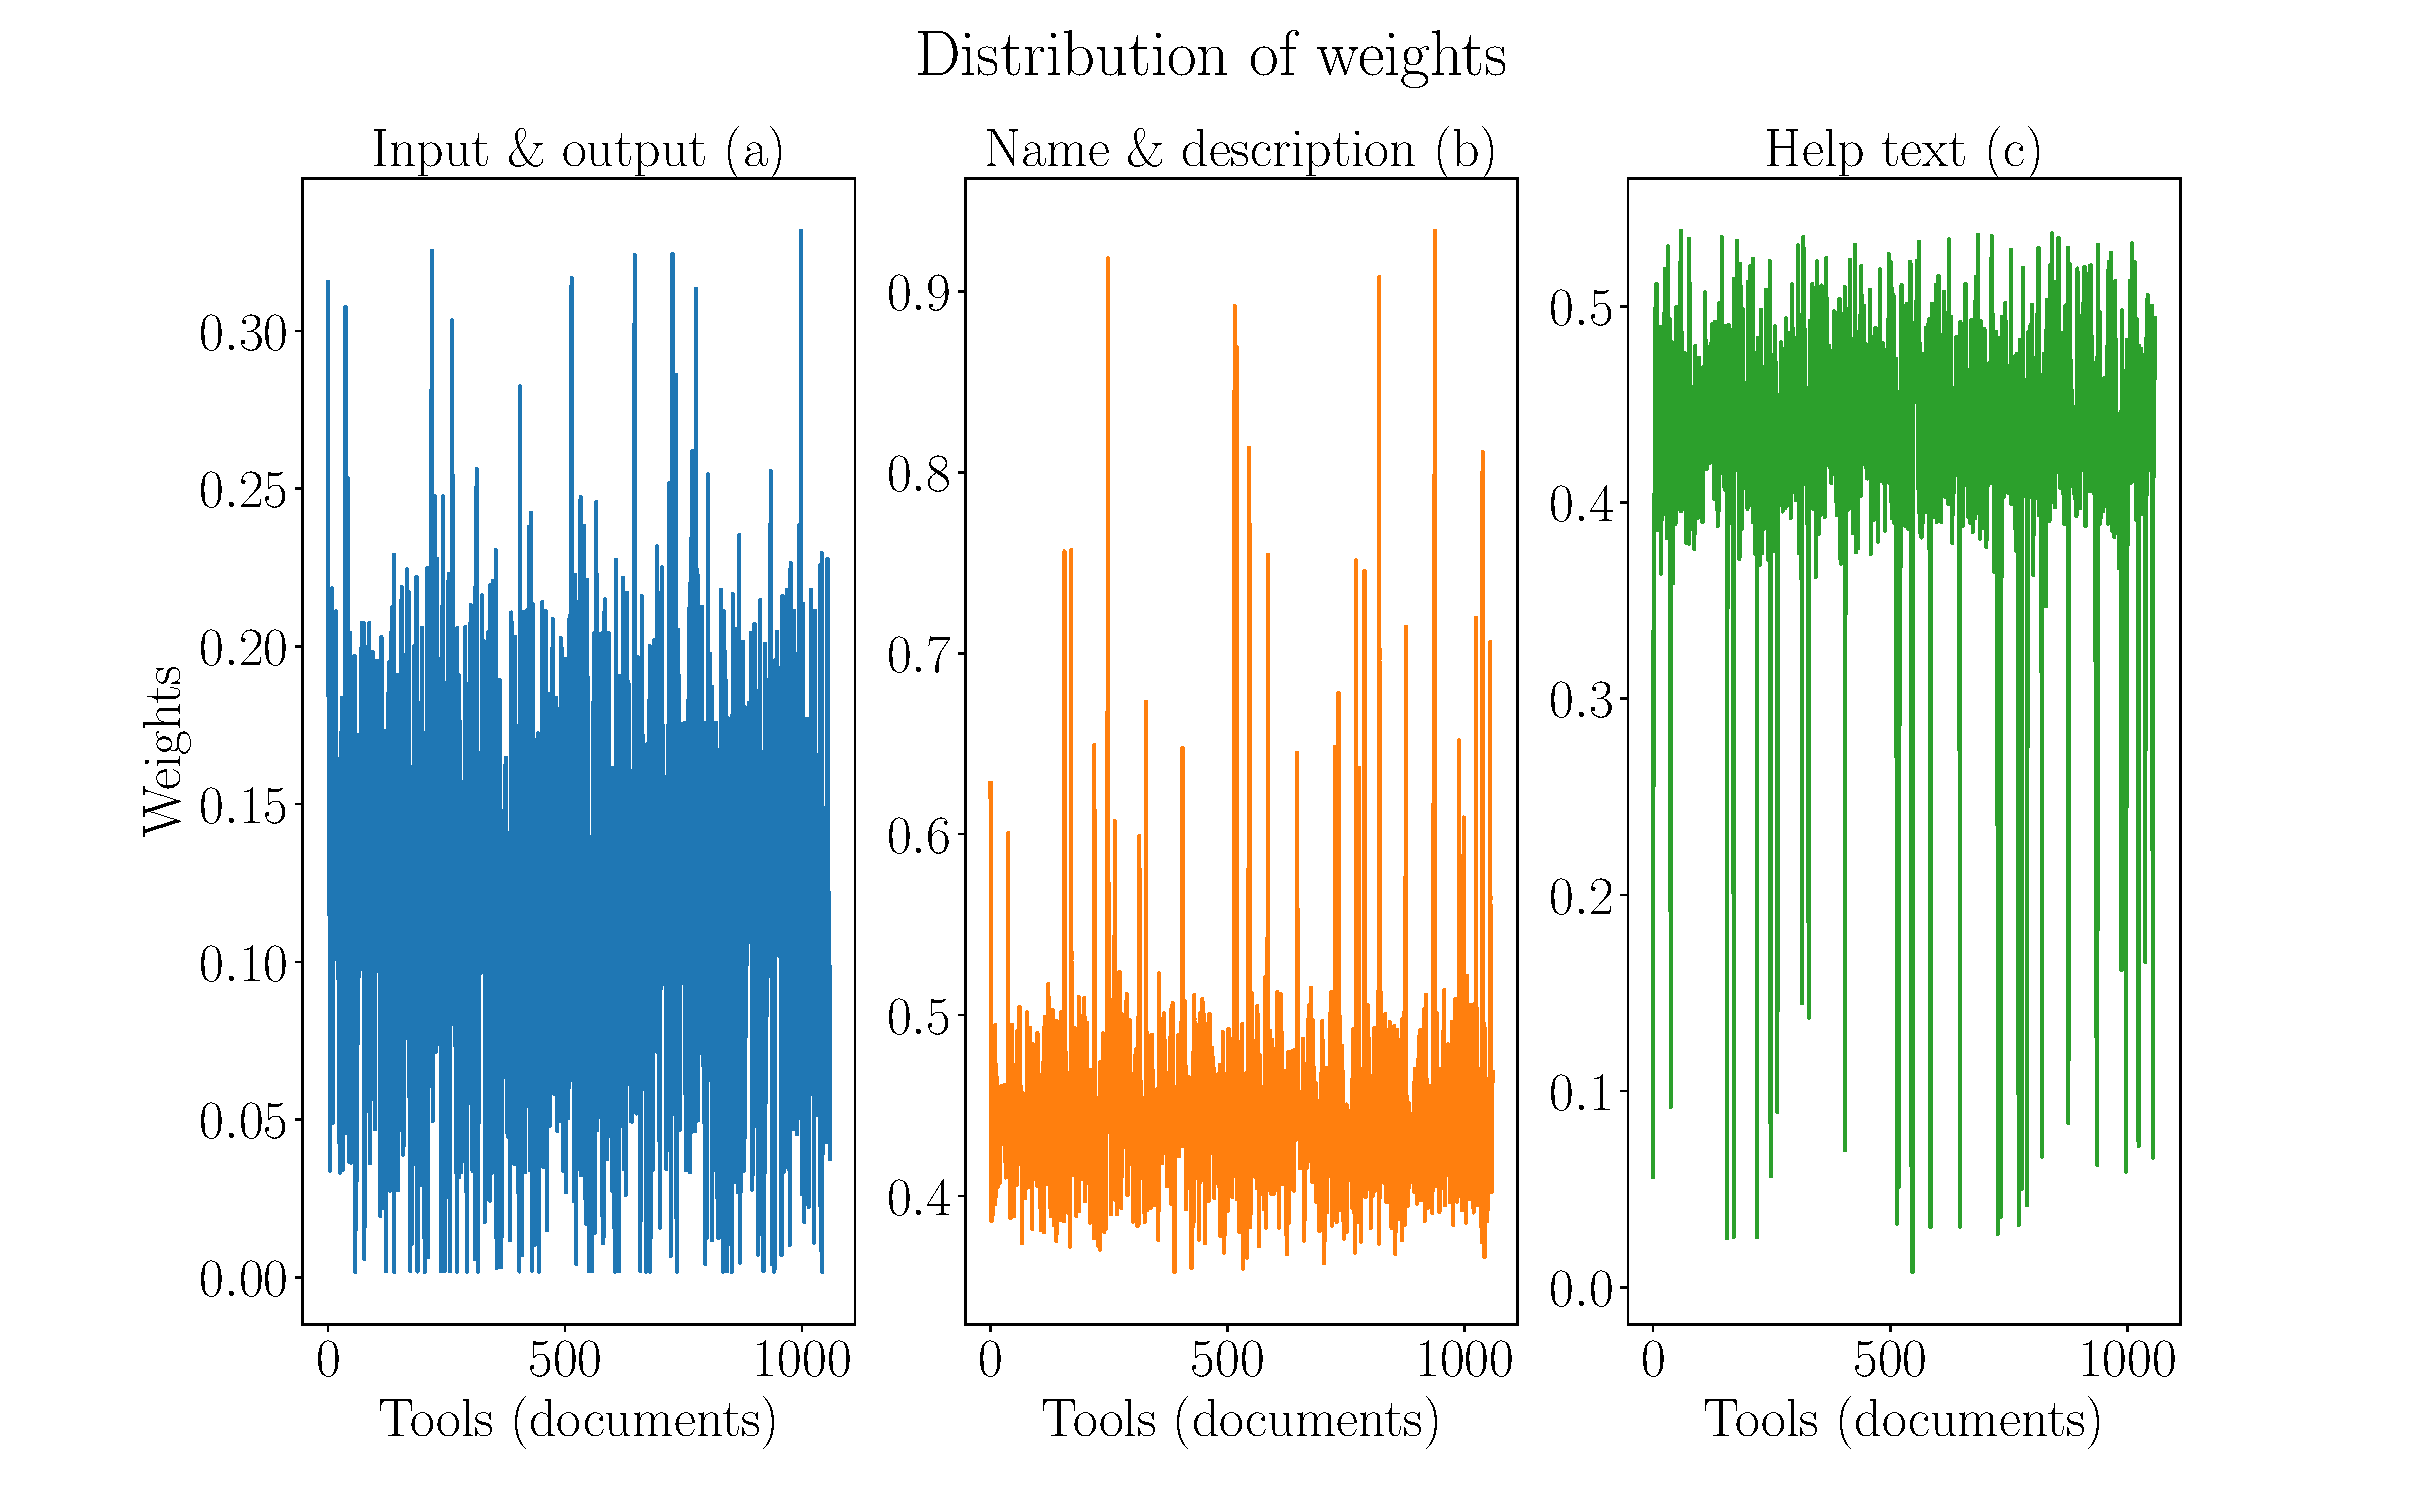
\includegraphics[scale=0.35]{figures/Weights_doc2vec.pdf}}
    \caption[Weights distribution for doc2vec]{\textbf{Weight distribution learnt using "paragraph vectors" approach}: this plot shows the distribution of weights for multiple tools attributes learnt using "paragraph vectors" approach. We can see that the magnitude of weights for input and output file types are lower compared to two other attributes. }
\end{centering}
\end{figure}


\subsection{Learning rate}

\begin{figure}[h]
\begin{centering}
    {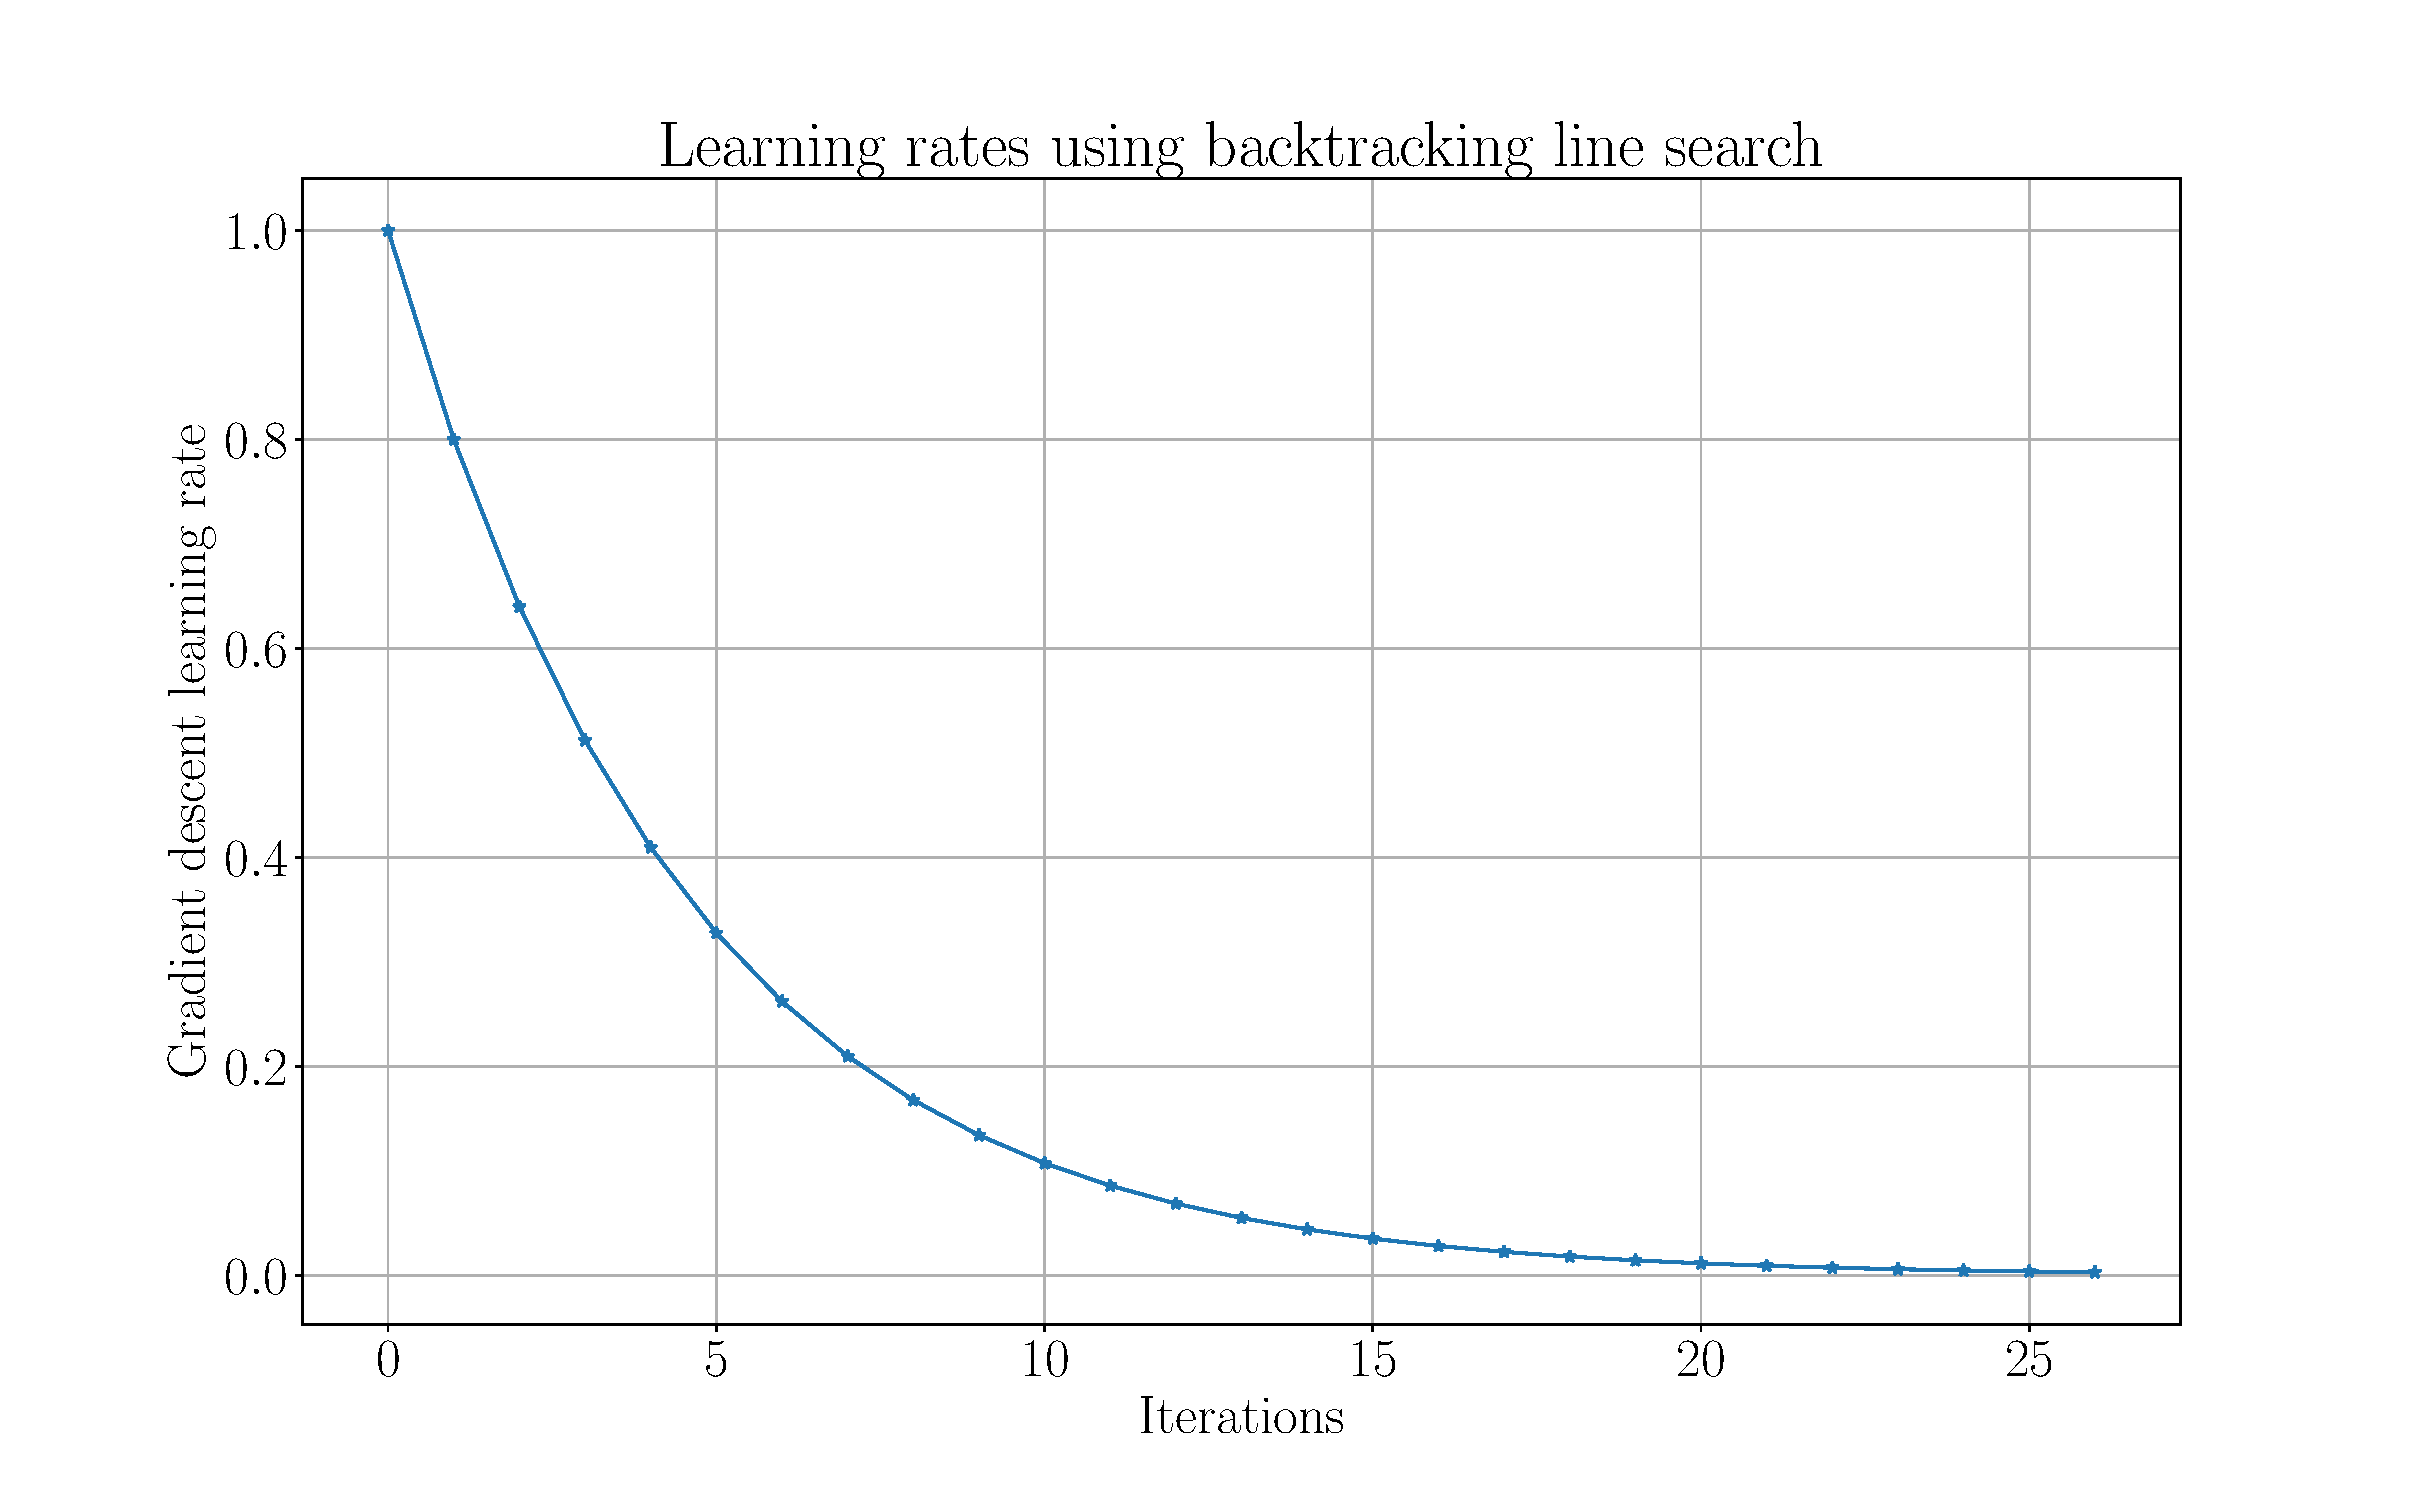
\includegraphics[scale=0.35]{figures/Learning_rates_LSI.pdf}}
    \caption[Weights distribution for doc2vec]{\textbf{Weight distribution learnt using "paragraph vectors" approach}: this plot shows the distribution of weights for multiple tools attributes learnt using "paragraph vectors" approach. We can see that the magnitude of weights for input and output file types are lower compared to two other attributes.}
\end{centering}
\end{figure}


\begin{figure}[h]
\begin{centering}
    {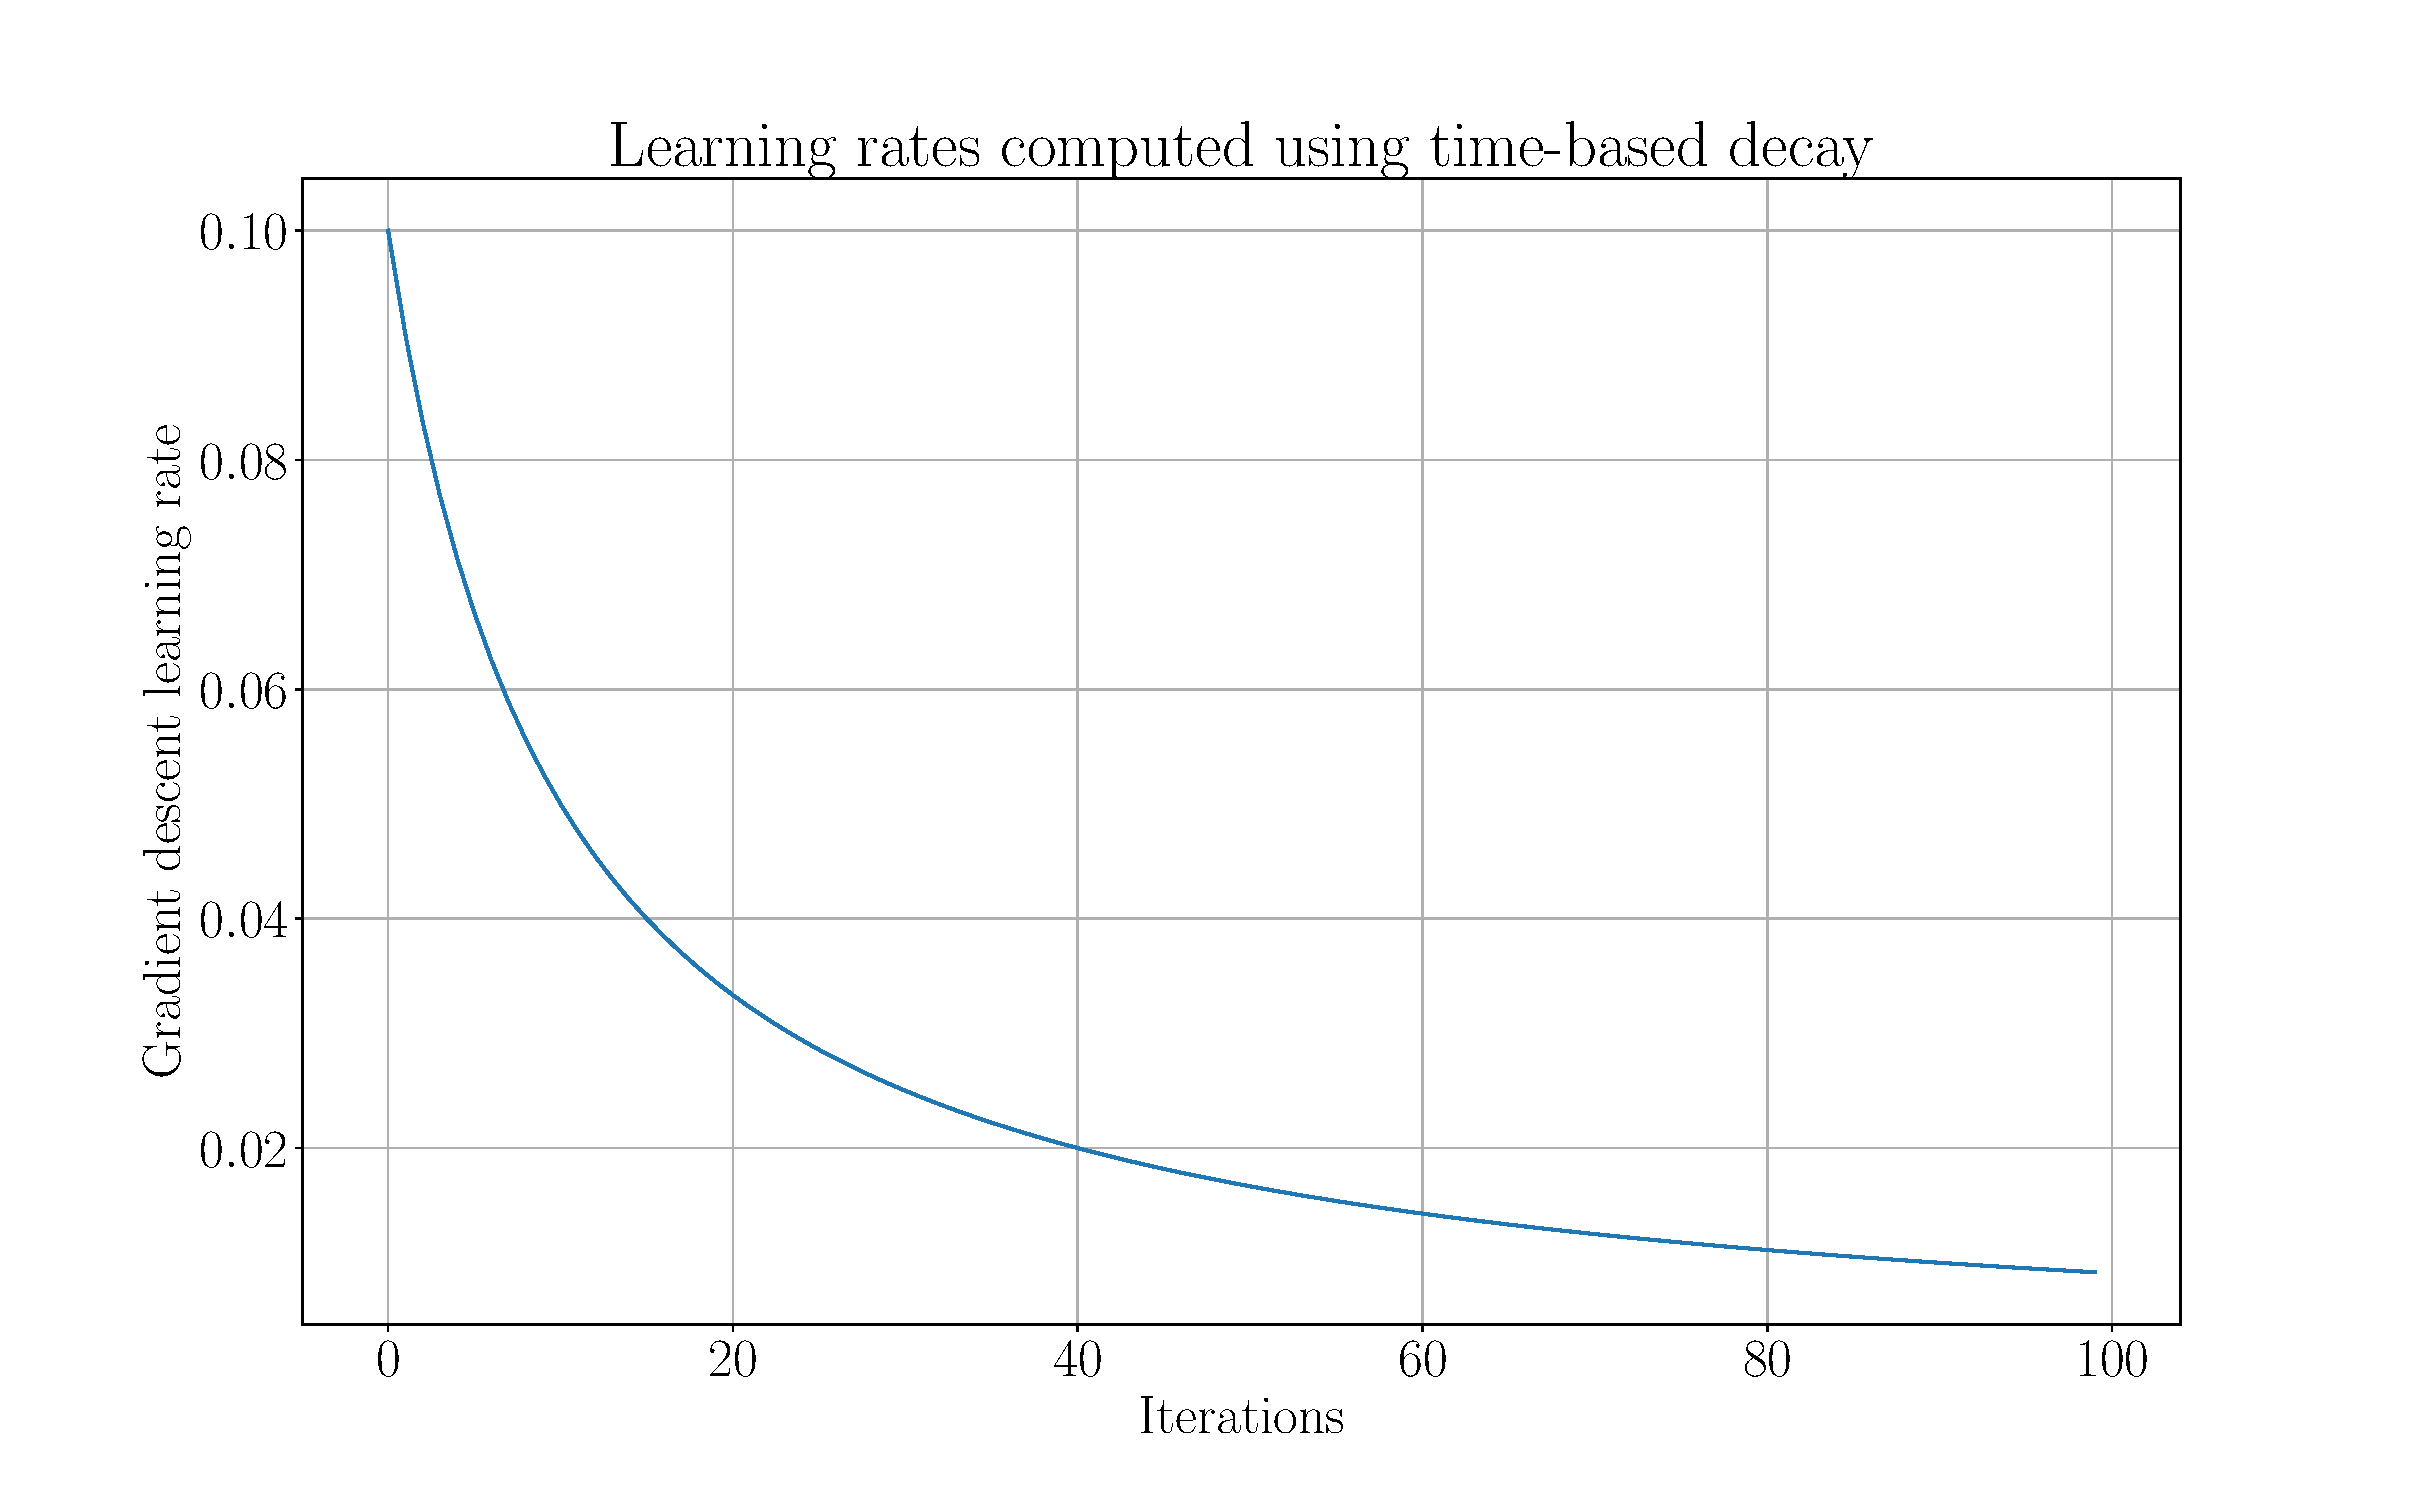
\includegraphics[scale=0.35]{figures/Learning_rates_PV.pdf}}
    \caption[Weights distribution for doc2vec]{\textbf{Weight distribution learnt using "paragraph vectors" approach}: this plot shows the distribution of weights for multiple tools attributes learnt using "paragraph vectors" approach. We can see that the magnitude of weights for input and output file types are lower compared to two other attributes.}
\end{centering}
\end{figure}


\subsection{Visualizer}
\subsection{LSI}
\subsection{Paragraph vectors}


